\documentclass[12pt]{article}
\usepackage{listings}
\usepackage{color}
\usepackage{biblatex}
\bibliography{Implementation.bib}
\definecolor{dkgreen}{rgb}{0,0.6,0}
\definecolor{gray}{rgb}{0.5,0.5,0.5}
\definecolor{mauve}{rgb}{0.58,0,0.82}
\usepackage[a4paper, total={6in, 9.25in}]{geometry}
%opening
\usepackage{xcolor}
\usepackage[]{algorithmic, algorithm, letltxmacro}
\usepackage{eqparbox}
\usepackage{titlesec}
\usepackage[]{graphicx}
\usepackage{array}
\usepackage{hyperref}
\usepackage{xcolor}
\usepackage{hhline}
\usepackage{geometry}
\hypersetup{
    colorlinks,
    linkcolor={red!50!black},
    citecolor={blue!50!black},
    urlcolor={blue!80!black}
}
\newlength{\commentindent}
\setlength{\commentindent}{.5\textwidth}
\makeatletter
\renewcommand{\algorithmiccomment}[1]{\unskip\hfill\makebox[\commentindent][l]{$\triangleright$~#1}\par}
\LetLtxMacro{\oldalgorithmic}{\algorithmic}
\renewcommand{\algorithmic}[1][0]{%
	\oldalgorithmic[#1]%
	\renewcommand{\ALC@com}[1]{%
		\ifnum\pdfstrcmp{##1}{default}=0\else\algorithmiccomment{##1}\fi}%
}
\newcommand{\minus}{\scalebox{0.75}[1.0]{$-$}}
\makeatother
\renewcommand\algorithmicrequire{\textbf{Input:}}
\renewcommand\algorithmicensure{\textbf{Output:}}

\setcounter{secnumdepth}{4}
\titleformat{\section}
{\normalfont\Large\bfseries}{\thesection}{1em}{}
\titleformat{\subsection}
{\normalfont\normalsize\bfseries}{\thesubsection}{1em}{}
\titleformat{\subsubsection}
{\normalfont\normalsize\bfseries}{\thesubsubsection}{1em}{}
\titleformat{\myparagraph}[runin]
{\normalfont\normalsize\bfseries}{\theparagraph}{1em}{}
\titleformat{\subparagraph}[runin]
{\normalfont\normalsize\bfseries}{\thesubparagraph}{1em}{}
\usepackage{collcell}
\newcolumntype{L}{>{\collectcell\lstinline}l<{\endcollectcell}}
\usepackage[font=small,skip=0pt,justification=centering]{caption}
\lstset{frame=tb,
  language=Python,
  aboveskip=3mm,
  belowskip=3mm,
  showstringspaces=false,
  columns=flexible,
  basicstyle={\small\ttfamily},
  numbers=none,
  numberstyle=\tiny\color{gray},
  keywordstyle=\color{blue},
  commentstyle=\color{dkgreen},
  stringstyle=\color{mauve},
  breaklines=true,
  breakatwhitespace=true,
  tabsize=3
  }
\hfuzz=5.002pt 
\usepackage{url}
\usepackage{subfigure}
\usepackage{multirow}
\usepackage{booktabs}
\usepackage{siunitx}
\usepackage{longtable}
%%% --- The following two lines are what needs to be added --- %%%
\setcounter{biburllcpenalty}{7000}
\setcounter{biburlucpenalty}{8000}
\graphicspath{ {./demographs/} {./insertion/} {./results} {./lengthgraphs} {./basegraphs} {./sortedgraphs} {./logo}}
\usepackage{tabularx}
\usepackage{adjustbox}
% \usepackage{}
\begin{document}
\pagenumbering{gobble}
    \begin{center}
      
    
    \includegraphics[draft=false,width=2.92358in,height=0.6639in]{logo}
    \vspace{2cm}
    \begin{LARGE}
      \linebreak
      COMP 390
      \vspace{.8cm}
      \linebreak
      \vspace{1.5cm}
      2023/24
      \linebreak     
      Integer sorting method for PyPy   
    \end{LARGE}
    \linebreak   
    \vspace{2.5cm}
    \begin{table}[h]
      \begin{large}
        
        \centering
        \begin{tabularx}{.7\linewidth}{Xr}
          
          Student Name: & William Dixon \\
          & \\
          Student ID: & 201434308\\
          & \\
          Supervisor Name: & Sebastian Wild
        \end{tabularx}
        
      \end{large}
      \end{table}
      \vspace{1cm}
      
    \begin{LARGE}
      
      DEPARTMENT OF\linebreak      
      COMPUTER SCIENCE
      \vspace{4.5cm}
      
    \end{LARGE}
    \begin{large}
      
      University of Liverpool
      
      Liverpool L69 3BX
    \end{large}
      
  \end{center}
  \pagebreak

\pagenumbering{arabic}
{
  \hypersetup{linkcolor=black}
  \tableofcontents
}
\newcommand{\myparagraph}[1]{\paragraph{#1}\mbox{}\\}
\pagebreak
\section{Abstract}
PyPy is a replacement for CPython that is built using RPython, the main reason to use it instead of CPython is that it generally runs faster. The goal of this project is to improve the speed PyPy by replacing the the sorting algorithm implemented by PyPy for lists of integers with Radix sort.
\par
PyPy currently uses Timsort, which is a comparison-based, stable sorting algorithm that takes $n\log{n}$ comparison to sort an array of $n$ elements in the worst case, it uses this algorithm for all lists regardless of the type of their elements but PyPy includes the functionality to apply different sort methods to lists containing different types. This project is centered around utilising an alternative sorting algorithm used by PyPy for lists of integers, which is based on the principle that a non-comparison-based, non-stable sorting algorithm is not necessary for sorting integers and that by exploiting this, a faster solution can be cfound. 
\par
Radix sort is a non comparison-based algorithm that takes $kn$ time in the worst case to sort a list of $n$ integers with $k$ refering to the number of digits. In this project it has been implemented using counting sort and pigeonhole sort as an integer sorting method as well as in the variations that sort digits decreasing from the most significant digit and increasing from the least significant.
\par
This project breaks down all operations of radix sort into their foundational components to understand the most optimal way to apply them to implementating the algorithm in PyPy and uses an extensive testing process to evaluate which of the methods is the most appropriate for use.
\pagebreak

\section{Design}
\label{sec:design}
	\subsection{Pseudocode}
	This is an implementation in pseudocode of the 4 components of the radix sort variations included in this project: Radix sort starting from the most significant and least significant digit and then the integer sorting methods Counting sort and Pigeonhole sort. Each permutation of Radix sort takes the input array \textit{A} of integers and treats each item \textit{A[i]} as a series of digits d within the range 0 \textit{$\leq$ d $<$ k} where \textit{k} is the radix or the number of unique integer keys. 
	\subsubsection{Integer Sorting}
	Integer sorting is a method of sorting a list off inputs by identifying the integer key of each value of the input and using that to identify it's position in the output. Because the sorting is performed based on the integer key and not based on comparisons to other list items, it is non-comparison-based. Integer sorting is the underlying sorting method that is applied to each digit of the input array.
	\myparagraph{Pigeonhole Sort}
	\label{ssec:pigeonhole}
	Pigeonhole sort operates by instantiating an array \textit{B} of length \textit{k} (1) containing empty arrays (3). The input array \textit{A} is iterated over and each item \textit{A[i]} is appended to the array in \textit{B} at t he position that corresponds to the current integer key of the current item. \textit{B} is then iterated over (10) and each item in each array overwrites the original array in order (11). 
	\begin{algorithm}[H] % enter the algorithm environment
		\caption{Pigeonhole Sort({A})} % give the algorithm a caption
		\label{alg1} % and a label for \ref{} commands later in the document
		\begin{algorithmic}[1] % enter the algorithmic environment#			
			\REQUIRE $A \Leftarrow$ Unsorted Array of length $n$ with maximum value $k$
			\ENSURE Sorted Array
			\STATE $B \Leftarrow [1..k]$ \COMMENT{Buckets array}
			\FOR{$i\gets 1$ to $k$}
			\STATE $B[i] \Leftarrow [$\space$]$ \COMMENT{Each bucket contains empty array}
			\ENDFOR
			\FOR{$j\gets 1$ to $k$}
			\STATE $append$\space$ A[j]$\space$ to$\space$ B[A[j]]$ \COMMENT{Move item to bucket}
			\ENDFOR
			\STATE $c \Leftarrow 1$ \COMMENT{Insertion index of items into A}
			\FOR{$i\gets 1$ to $k$}
			\FORALL{$item$ in $B[i]$}
			\STATE $A[c] \Leftarrow item$ \COMMENT{Move items from bucket to A}
			\STATE $c \Leftarrow c + 1$		\COMMENT{Increment insertion index}
			\ENDFOR
			\ENDFOR
			\STATE \textbf{return} $A$
		\end{algorithmic}
	\end{algorithm}

	\pagebreak
	\myparagraph{Counting Sort}
	\label{ssec:counting}
	Counting sort instantiates 2 arrays; \textit{B}, the output array equal in length to the input array \textit{A} (1), and \textit{C}, a count array to store the frequency of each integer key of length \textit{k}. \textit{C} is instantiated containing only integers of value 0 (2, 4). The input array is iterated over and the integer in C at the position equal to the current integer key of the current item is incremented (7), producing a histogram of the frequency of each key. This count list is then accumulated such that each item is added to the sum of the previous items (10). Finally the input array is iterated over in reverse and each item is moved to the output array in the position that is referred to by the value expressed in the count array at the position of the current key of the current item(13), to ensure that values to not overwrite one another in the output array each item in the count array is decremented when a position in the output array is taken from it (14).
	\begin{algorithm}[H]
		\caption{Counting Sort({A})}
		\label{alg2}
		\begin{algorithmic}[1]					
			\REQUIRE $A \Leftarrow$ Unsorted Array of length $n$ with maximum value $k$
			\ENSURE Sorted Array
			\STATE $B \Leftarrow [1..n]$ \COMMENT{Output array}
			\STATE $C \Leftarrow [1..k]$ \COMMENT{Count array}
			\FOR{$i\gets 1$ to $k$}
				\STATE $C \Leftarrow 0$
			\ENDFOR
			\FOR{$j\gets 1$ to $n$}
				\STATE $C[A[j]] \Leftarrow C[A[j]] + 1$ \COMMENT{Count occurrence of value}
			\ENDFOR
			\FOR{$i\gets 2$ to $k$}
				\STATE $C[i] \Leftarrow C[i] + C[i-1]$\COMMENT{Accumulate Count array}
			\ENDFOR
			\FOR{$j\gets n$ to $1$ by $-1$}
				\STATE $B[C[A[j]]] \Leftarrow A[J]$ \COMMENT{Move item from input to output array}
				\STATE $C[A[j]] \Leftarrow C[A[j]] - 1$ \COMMENT{Decrement count array}
			\ENDFOR
			\STATE \textbf{return} $B$
		\end{algorithmic}
	\end{algorithm}	
	\pagebreak
	\subsubsection{Radix Sort}
	Radix sort is the method of applying the integer sorting method to each digit of the input, there are two approaches to this: Least significant digit first (LSD) or Most significant digit first (MSD).
	\myparagraph{Least Significant Digit}
	\label{ssec:lsd}
	Least Significant Digit Radix sort (LSD) takes an input array \textit{A} and sorting function \textit{f()} which can be either of the previous integer sorting methods. The input array is sorted via the chosen method once for each digit in the chosen radix of the largest absolute value \textit{m} (3).
	\par 
	This sorting process is applied first at the least significant or rightmost digit and progresses incrementally to the most significant or leftmost digit. Values can have an unequal number of digits provided any digits farther left than their most significant are taken as 0.
	
	\begin{algorithm} % enter the algorithm environment
		\caption{LSD({A, f()})} % give the algorithm a caption
		\label{alg3} % and a label for \ref{} commands later in the document
		\begin{algorithmic}[1] % enter the algorithmic environment#			
			\REQUIRE $A \Leftarrow$ Unsorted Array of length $n$ with maximum absolute Value $m$
			\REQUIRE $f() \Leftarrow $Sorting function \COMMENT{Pigeonhole or Counting Sort}
			\ENSURE Sorted Array
			\STATE $d \Leftarrow$ Number of digits of m \COMMENT{Varies based on radix chosen}
			\STATE $A(i) \Leftarrow$ i-th digit of each item in A
			\FOR{$i\gets 1$ to $d$}
				\STATE $A \Leftarrow f(A(i))$ \COMMENT{Sorts Array using sort function}
			\ENDFOR
			\STATE \textbf{return} $A$
		\end{algorithmic}
	\end{algorithm}
	\pagebreak
	\myparagraph{Most Significant Digit} \label{sssec:msdradix}
	Most Significant Digit Radix sort (MSD) takes an input array \textit{A}, sorting function \textit{f()} and current digit \textit{i} which for the first call of the function should be the number of digits of the largest value in the input. This algorithm operates recursively, and the termination condition occurs when \textit{i} is equal to 0 meaning that all digits of the input have been sorted (1,2). After ensuring the termination condition has not been met the input array \textit{A} is then sorted using the chosen function with respect to the current digit (5). 
	\par 
	The input array is then iterated over and items that have an equal integer key value at the current digit are identified (8) and taken as a slice of the input array. This slice is then sorted recursively using a function call to \textit{MSD()} with a decremented value for \textit{i} meaning they are sorted over the next least significant digit (11). Once the termination condition has been reached within this slice and all sub-slices created by recursive calls the algorithm resets the start point of the slice and identifies further slices to sort (12). Each slice on which \textit{MSD()} is called that does not meet the termination condition must wait until all sub-lists return, which are then placed together in \textit{A} and finally returned (15).
	\begin{algorithm} % enter the algorithm environment
		\caption{MSD({A, i, f()})} % give the algorithm a caption
		\label{alg4} % and a label for \ref{} commands later in the document
		\begin{algorithmic}[1] % enter the algorithmic environment#			
			\REQUIRE $A \Leftarrow$ Unsorted Array of length $n$ with maximum absolute Value $k$
			\REQUIRE $i \Leftarrow$ Digit to sort Array on \COMMENT{start with number of digits of k}
			\REQUIRE Sorting function $f()$\COMMENT{Pigeonhole or Counting Sort}
			\ENSURE Sorted Array
			\IF{$i==0$}
				\STATE \textbf{return} $A$
			\ENDIF
			\STATE $A(i) \Leftarrow$ i-th digit of each item in A
			\STATE $A \Leftarrow f(A(i))$ \COMMENT{Sorts Array using sort function}
			\STATE $s \Leftarrow 1$ \COMMENT{Starting position of recursive call}
			\FOR{$j\gets 1$ to $s$}
				\IF{$A(i)[j] == A(i)[s]$}
					\STATE Do Nothing
				\ELSE
					\STATE $A[s..j-1] \Leftarrow MSD(A[s..j-1](i), i-1)$
					\STATE $s \Leftarrow j$ \COMMENT{Reset start position of array slice}
				\ENDIF
			\ENDFOR
			\STATE \textbf{return} $A$
		\end{algorithmic}
	\end{algorithm}
	\pagebreak
	\subsection{Time complexity}
	\label{ssec:timecomplexity}
	\subsubsection{Integer Sorting}
	Counting and Pigeonhole sort both require one iteration over the input list which contains $n$ items and one pass over the intermediary buckets array for pigeonhole sort or the count array for counting sort, both of these arrays contain $k$ items where $k$ is the maximum range of input values. The combination of these two passes gives both integer sorting methods a time complexity of 
	\begin{table}[!h]
		\begin{center}
			\begin{tabular}{c}
				$\mathcal{O}\textit{(n+k)}$ 
			\end{tabular}				
			\end{center}
		\end{table}
	\subsubsection{Radix Sort}
	Radix sort repeatedly applies integer sorting to each successive digit of the input array, it differs from counting sort in that it does not sort into \textit{k} buckets but a constant base \textit{b} is chosen. It repeats the integer sorting method \textit{d} times where \textit{d} is the number of passes necessary to sort each digit of the maximum value in the input with respect to the base \textit{b} and can be expressed as \textit{d = $log_b$k}, giving a time complexity of:
	\begin{table}[!h]
		\begin{center}
			\begin{tabular}{c}

	 $\mathcal{O}$\textit{((n + b) $\cdot$ d)}
 \\ \\
	or if \textit{b} is a constant:
\\	\\
	$\mathcal{O}$\textit{(n $\cdot$ d)} 
			\end{tabular}
				
			\end{center}
		\end{table}
			
	However, in the application of this project, radix sort will only be applied to integers represented in 64-bits, meaning there is a defined upper bound to the max value \textit{k}. This is important because it means that that \textit{k} is polynomial in \textit{b} or that \textit{k} is always able to be represented by \textit{b} raised to some exponent \textit{c} where \textit{c} is some constant value. This can be expressed in the form \textit{k $=$ b$^{\mathcal{O}(1)}$} or \textit{$\mathcal{O}(1) = log_b$k}
	\par
	$\mathcal{O}(1)$ can be substituted in for \textit{d} in the time complexity analysis meaning Radix sort will run in $\mathcal{O}(n)$ or linear time in the context of this project.
	\pagebreak
	\subsection{Radix Selection}
	
	\label{sec:radixselection}
	Radix sort utilizes multiple rounds of integer sorting across the digits of the input list, therefore, it is important to create an effective method of separating an integer into its component digits. When expressing a number, requires the selection of a numerical base, this is the number of unique values that can be displayed in each digit. When a value exceeds the maximum value within this base, another digit must be added; i.e. in standard decimal or base 10 numbers 0 through 9 can be expressed in a single digit but increasing beyond this range requires adding a second digit to create the number 10.
	\par
	Though numbers in typical day to day use by humans are typically thought of as Arabic numerals in the decimal system, this is a social convention which this algorithm is not beholden to, and as Radix sort fundamentally relies on the processing of the component digits of an integer it is of great importance to select an appropriate base as well as identify an efficient method for processing each digit.
	\subsubsection{Explanation}
	\label{ssec:radixexplanation}
	Python stores integers in the format "two’s complement”, which is a type of binary and therefore uses a base of 2. This means that bases that are of the order $2^b$ where $b$ is some integer are the most suitable for this project as each single $2^b$ digit utilizes a maximum of $b$ bits and each subsequent digit utilizes the next $b$ bits.
	\par
	The main consideration when selecting a numerical base for Radix sort is the trade off between iterations of the integer sorting method, minimized by selecting a higher base, and speed of each iteration of integer sorting, minimized by selecting a lower base. There is technically no upper bound for $b$ when taking a theoretical approach, however in practice the constraints of a physical memory limit and larger overhead costs limit radix sort algorithm to reasonably small values of $b$. This project includes values in the range $[2..16]$ as a value of $18$ (and presumably anything above) performed so poorly the charts generated were unreadable for any other base.
	\par 
	The reason performance suffers with a higher radix being used is that each item in the range $[1..b]$ represents an item in the bucket list or count list (depending on integer sorting method) and each list item requires a memory address and a certain allocation of memory when being instantiated, each list item requires access to a location in the count list/bucket list during the building stage and the count/bucket list requires iterating over when rebuilding the input list. Whilst a higher value of $b$ is desirable to reduce iterations over the input, any increase causes an exponential increase in the these overhead costs incentivizing a lower $b$. 
	\par 
	The effect of larger values of $b$ being more costly is highlighted further when considering the effect of cache misses on performance. A cache is a small piece of high speed memory that can be accessed much faster than main memory, however this memory is much smaller than main memory and so can only store limited amounts of data. The number of successful reads of a count/bucket list item from cache can greatly improve the performance of an algorithm, and when considering radix sort, a higher $b$ value decreases the ability of the system to be stored in the cache. Lamarca and Ladner use a $b = 16$ in their implementation of radix sort to minimize cache misses and instruction count \cite{LAMARCA199966}.
	\subsubsection{Implementation}
	The method of identifying each digit of an integer from the binary representation first involves manipulating the integer such that the desired digit is in the rightmost position, in base $b$ this means discarding the rightmost $n \cdot d$ binary digits where d is the index (from the right) of the required digit in base $2^b$. Following this, isolating the rightmost $b$ binary digits produces the correct digit.  
		\par
	In order to complete this task, bitwise operations have been utilized (see \ref{ssec:bitwise}).


	\begin{table}[!htb]
		\centering
		
		\vspace{0.3cm}
		\setlength{\tabcolsep}{1pt}		
        \begin{tabular}[t]{cccc}			
			\rotatebox{90}{\begin{math}
				\left\{
				  \begin{array}{l}
					\rotatebox[origin=c]{-90}{1}\\
					\rotatebox[origin=c]{-90}{1}\\
					\rotatebox[origin=c]{-90}{1}\\
					\rotatebox[origin=c]{-90}{0}
				  \end{array}
				\right.
			  \end{math}}		
			  &
			  \hspace{5pt}
			  \rotatebox{90}{\begin{math}
				\left\{
				  \begin{array}{l}
					\rotatebox[origin=c]{-90}{1}\\
					\rotatebox[origin=c]{-90}{0}\\
					\rotatebox[origin=c]{-90}{1}\\
					\rotatebox[origin=c]{-90}{0}
				  \end{array}
				\right.
			  \end{math}}
			  &
			  \hspace{5pt}
			  \rotatebox{90}{\begin{math}
				\left\{
				  \begin{array}{l}
					\rotatebox[origin=c]{-90}{0}\\
					\rotatebox[origin=c]{-90}{1}\\
					\rotatebox[origin=c]{-90}{1}\\
					\rotatebox[origin=c]{-90}{0}
				  \end{array}
				\right.
			  \end{math}}
			  &
			  \hspace{5pt}
			  \rotatebox{90}{\begin{math}
				\left\{
				  \begin{array}{l}
					\rotatebox[origin=c]{-90}{0}\\
					\rotatebox[origin=c]{-90}{0}\\
					\rotatebox[origin=c]{-90}{0}\\
					\rotatebox[origin=c]{-90}{0}
				  \end{array}
				\right.
			  \end{math}}
			  \\
			 Digit 4 & \hspace{10pt} Digit 3 & \hspace{10pt}Digit 2 & \hspace{10pt}Digit 1 \\
			   14 & \hspace{10pt}10 & \hspace{10pt} 6 & \hspace{10pt}0
			
        \end{tabular}%
		\vspace{0.1cm}
		\caption*{The 4 digits in base $2^4$ of a 16 bit integer: $60000$}

	\end{table}
	\subsection{Negative Integers}
	\label{ssec:negativeintegers}
	\subsubsection{Two's Complement}
	\label{ssec:negativestwos}
	When handling integers in two’s complement, positives are represented in binary, but with a leading 0 in the leftmost position to indicate the positive sign of the integer. Negative integers are represented with a leading 1 which represents that the binary value of this digit is to be subtracted i.e. negative and all other binary digits are positive such that the sum of all the digits equals the integer being represented. table reference has been included to illustrate this, as you can see the value $+3$ has a leading $0$ at index $2$, representing $2^{2}$ is not subtracted, this is followed by 1 in all remaining digits representing the addition of $2^{1}$ and $2^{0}$ or $2+1=3$. $\minus3$ is represented by a leading 1 to represent $\minus2^{2}$ followed by 0 1 to represent no addition of $2^{1}$ and the addition of $2^{0}$ or $\minus4 + 1 = \minus3$.
	\par
	The effect of performing Radix sort using bitwise methods without any accommodation for negativity is that due to their leading 1, negative values will be incorrectly sorted as though they are larger than positive values. They will also be sorted into the correct order relative to other negative values (increasing from most negative to least negative), as can be seen in \hyperref[table:twoscomplement]{Table 1}, which is sorted. 	
	\par
	\subsubsection{Negatives in RPython}
  	\label{ssec:pypynegatives}
	Because the purpose of this project was to incorporate this sorting algorithm into the standard library for Pypy, it had to be written in RPython, the language used for Pypy. RPython is a restricted form of python, specifically it is a form of Python 2, which is relevant to the handling of integers as RPython inherits Python2’s method of allocation of a quantity of bits for each integer equal to the machine word size of the system  it is being run on (typically this is 32 or 64 bits), even if the integer can be expressed in fewer bits. The leftmost bit represents the sign of the integer and the remaining bits between the sign bit and the most significant bit are copies of the sign bit. To put this in the context of two’s complement, this representation can be understood as the first bit representing a value of $\minus2^{m}$ where m is the machine word length and all following digits are additions of machine where n is the index of the bit counted from the rightmost bit and in the range $[(m-1)..0]$, the sum of these values is the value of the integer.
	\par

	This project handles digits with a radix of $2^{b}$ with $b$ being some integer, and in binary representation this means each digit requires $b$ bits. This causes challenges when handling negatives as the most significant digit of integers that are made up of a number of bits not divisible by $b$ includes sign bits and integers that are made up of a number of digits divisible by $b$ do not include a sign bit.

	\subsubsection{Solution}
	The approach used in this project was to identify the number of digits needed to express the largest absolute value of the input in the chosen base and then use a bitwise exclusive or (\ref{sssec:xor}) to flip all bits to the left of it. The effect of this is that when performing a radix sort across all 64 bits of the integer list is that the order is now corrected as negative values closer to 0 retain their higher position relative to more negative values but are now always sorted below positive values.
	\par
	In order to reduce unnecessary iterations, radix sort only iterates a number of times such that the number of bits sorted across is at minimum the number of bits needed to express the absolute maximum value of the list including 1 sign bit, rounded up of course to the nearest multiple of $b$. In cases where the number of bits needed is divisible by $b$, it means the algorithm performs an addition iteration exclusively on sign bits whereas in the inverse case there is no increase in iteration count. 

	\begin{table}[!h]
		\vspace{0.5cm}
		\begin{center}
			\begin{tabular}{|c c c|} 
				\hline
				Bits & Unsigned Value & \begin{tabular}{c}Signed Value\\(Two's Complement)\end{tabular}\\
				\hline\hline
				000 & 0 & 0  \\ 
				\hline
				001 & 1 & 1  \\
				\hline
				010 & 2 & 2  \\
				\hline
				011 & 3 & 3  \\
				\hline
				100 & 4 & -4  \\ 
				\hline
				101 & 5 & -3  \\  
				\hline
				101 & 6 & -2  \\ 
				\hline
				111 & 7 & -1  \\ 
				\hline
			\end{tabular}
			\vspace{0.5cm}
			\caption{3 bit integers and their respective values when interpreted in unsigned binary and two's complement}
			\label{table:twoscomplement}
		\end{center}
	\end{table}
\pagebreak
\section{Implementation}
\subsection{Extra Methods and Classes}
The algorithm relies upon a number of helper methods to operate effectively and must be contained in a specific class structure to allow for it's inclusion into PyPy. This section explains the structure of the class used and contains documentation for all of the helper methods that are used by the algorithms.

\subsubsection{Function absolute}
Allows for the calculation of absolute values without overflow issues specifically caused by using the minimum possible value as the positive of this value requires an extra bit to express and thus causes an overflow error.
\begin{lstlisting}
	import sys
        
	def absolute(num):
        if num == (-sys.maxint) - 1:
			return sys.maxint
        return -num if num < 0 else num
\end{lstlisting}

\subsubsection{Function make\textunderscore radixsort\textunderscore class}
The container function that instantiates all other functions, this is modeled on the existing function in listsort.py \cite{listsort} to minimize compatibility issues when including this project in the PyPy library.
\begin{lstlisting}
    def make_radixsort_class(
        setitem=None,	setslice=None,
    ):
  \end{lstlisting}
\subsubsection{Functions setitem and setslice}
These functions have been imported from the existing listsort.py file within rlib \cite{listsort}. They enable the input list to be edited by functions within the Radixsort class. When the $.sort()$ function is called by PyPy, it initializes the Radixsort class with the list as a constructor, this means that the list attribute is not mutable from within the class unless these functions are imported.
\begin{lstlisting}
    if setitem is None:
      def setitem(list, item, value):
          list[item] = value
	
	if setslice is None:
		def setslice(list, slice, index):
			list[index : index + len(slice)] = slice
  \end{lstlisting}


\pagebreak
\subsubsection{Function int\textunderscore digits}
\label{ssec:intdigits}
Returns the quantity of digits needed to express an integer using a specified numerical base. Each digit requires $b$ binary bits to express an integer in the base $2^b$ excluding the sign bit which is not factored in when calculating the return value of this function but is accounted for elsewhere (see \ref{sssec:listmaxdigits}).
\par
This function repeatedly rightshifts the input value by a number of bits starting at the chosen base and increasing by the same on each repeat. This is performed until the right shifted input is equal to $0$ or $-1$ if the input is positive or negative respectively, which indicates that the number of bits the input has been shifted by are equal to or greater than the number of bits needed to express it. The number of repeats (\textit{l}) is returned as this represents the number of digits needed to express the input value.
\par
On each repeat the current value for the right shifted input is compared to the next value to ensure that the next value is closer to $0$, this is done because in RPython right shifting an input by \textit{n} actually performs the input right shifted by the \textit{n modulo s}, where \textit{s} is the machine word size. For inputs occupying a number of bits in the range $s-b < s$, the smallest value by which the input must to be shifted that exceeds or equals the number of bits of the input is greater than \textit{s}, triggering the modulo operation and thus resulting in a larger value than the previous iteration of the loop and thus the exit condition of the loop is never met. Due to these factors an extra exit condition has been included should the next right shifted input value be further from 0 than the current one.
\par
Intuitively it would seem the use of logarithms would be a more prudent and concise way of performing this function, as taking $\log _{r} i$ (where \textit{r} is the chosen radix) and rounding up would give the same result as this function. However the inbuilt logarithm function of RPython does not allow the base to be specified forcing the use of $\frac{\log i}{\log r}$. Implementation of this solution caused occasional floating point errors when rounding, these errors occasionally allowed an incorrect calculation of a bit mask resulting in an incorrect sort, namely when the machine word length and number of bits of the input value were divisible by the chosen base without remainder. Whilst this situation is extremely rare and it was possible to hard-code a solution for these cases, including a systematic calculation error in a function was deemed too risky.
\begin{lstlisting}
	def int_digits(i, base):
		l = 1
		v = 0 if i >= 0 else -1
		prev = i >> (l * base)
		while prev != v:
			l += 1
			new = i >> (l * base)
			if absolute(new) < absolute(prev):
				prev = i >> (l * base)
			else:
				return l
		return l
\end{lstlisting}
\pagebreak


\subsubsection{Class Radixsort}
This is the class that contains all other functions of the radix sort algorithm. It is initialized with the input list which is stored as an attribute for access by other functions as well as the base and radix.\par
\par
The functions $setitem$ and $setslice$ are imported here as mentioned above so that the list can be edited outside of the scope of the class.
\begin{lstlisting}
        class Radixsort(object):
            def __init__(self, list, listlength=None):
                self.list = list
                self.base = 0
                self.listlength = len(self.list)
                self.radix = 0
    
            def setitem(self, item, value):
                setitem(self.list, item, value)
				def setslice(self, slice, index=0):
					setslice(self.list, slice, index)
      \end{lstlisting}

\subsubsection{Function list\textunderscore abs\textunderscore max}
This function returns the largest absolute value of the input list as well as identifying whether the list is sorted in ascending or descending order. These functions are combined as a time saving measure as they both require a pass over the data.
\par
The primary purpose of this function is to return the value that is used to identify the number of passes over the input necessary for sorting, this is the value that will contain the most digits and is thus the largest absolute value. 
\par
The secondary purpose of the function is to identify on the first pass over the list whether it is sorted, in which case the algorithm terminates, or if it is reverse sorted in which case the list is reversed and then the algorithm terminates.
\begin{lstlisting}
        self.ordered = True
        self.reverseOrdered = True
        def list_abs_max(self, checkorder=False):
            assert len(self.list) != 0
            m = self.list[0]
            n = self.list[0]
            prev = self.list[0]
            for i in xrange(1, len(self.list)):
                if self.list[i] > m:
                    m = self.list[i]
                if self.list[i] < n:
                    n = self.list[i]
					self.ordered &= self.list[i] >= prev
					self.reverseOrdered &= self.list[i] <= prev
					prev = self.list[i]
            return m if absolute(m) > absolute(m) else n
      \end{lstlisting}
\pagebreak
\subsubsection{Function insertion\textunderscore sort}
This is an implementation of insertion sort, it is used in MSD sorts when the length of a sub list falls below the critical value. This value was determined by testing demonstrated in \ref{sssec:insertiontesting}
\begin{lstlisting}
        def insertion_sort(self, start, end):
            for step in xrange(start, end):
                key = self.list[step]
                j = step - 1
                while j >= 0 and key < self.list[j]:
                    self.setitem(j + 1, self.list[j])
                    j = j - 1
                self.setitem(j + 1, key)
      \end{lstlisting}

\subsubsection{Function reverse\textunderscore slice}
This reverses the items of the input in between the provided start and stop indexes. By default is reverses the entire list, but includes provisions to reverse a smaller slice of the list (this was from an earlier version of the algorithm, this feature is currently unused).
\begin{lstlisting}
        def reverse_slice(self, start=0, stop=0):
            if stop == 0:
                stop = self.listlength - 1
            while start < stop:
                i = self.list[start]
                j = self.list[stop]
                self.setitem(start, j)
                self.setitem(stop, i)
                start += 1
                stop -= 1
      \end{lstlisting}
\pagebreak
\subsection{Bitwise operations}
\label{ssec:bitwise}
Bitwise operations operate on binary numerals at the level of individual bits, they allow for fast and consistent manipulation that bypasses arithmetic functions. Through the use of bitwise operations, radix sort can be performed using different numeral bases, meaning a different maximum value at each digit and a different total number of digits. By reducing the number of digits the amount of iterations over the data is reduced thereby improving run time, however this comes at the cost of an increase in the amount of time each round of integer sorting takes and an increase in the memory consumption due to the larger count list or quantity of bins. 
\par
Bitwise operations are particularly useful in this regard as it makes processing integers in bases of the order $2^b$ where $b$ is some integer very easy (see section \ref{ssec:radixexplanation}) whereas changing base from the standard base 10 requires time consuming arithmetic methods such as euclidean division.
\par
In order to properly implement bitwise operations it was necessary to properly explore their implementation in RPython as well as the implementation of the Integer type. In RPython each integer is comprised of exactly 64 bits, where 1 bit is assigned to represent the integer's sign, leaving a maximum of 63 bits to express the magnitude of the integer, this gives integers in RPython a range of $[\minus2^{63}$ $..$ $2^{63}\minus1]$. The PyPy interpreter considers any integer outside of this range to instead be of the `Long' type, and as such a list containing even a single value outside of this range does not have the Integer specific sorting method applied to it, thus values outside of this range are not within the scope of this project.
\par
I have already covered in general terms how these  are used in this project to identify the value of each digit in section \ref{sec:radixselection} and handle negative integers in \ref{ssec:pypynegatives} but in this section I will cover the implementation of the bit shift operations used in RPython.
\subsubsection{Left shift}\
\label{sssec:leftshift}
A `Left shift' refers to moving each bit of an integer a number of digits to the left, in RPython this is performed using: $i << s$ where $i$ is the integer to be shifted and $s$ is the number of digits the integer should be shifted to the left.
\par
RPython utilizes Arithmetic Shifting, this means when a shift is performed and the rightmost bit is no longer in the rightmost position, all digits in the range $[0 .. s]$ are overwritten with the value 0 and an equal quantity of digits in the leftmost positions are discarded.
\par
In this project, left shifting is used to create integers that occupy a specific number of bits and is used for the accommodations necessary to sort negative integers (further explained in \ref{sssec:xor}). 
\par

\begin{table}[htpb]
	\centering
\begin{tabular}{r|rrrrrrrr}
	
	\hline
	 Value   &   7 &   6 &   5 &   4 &   3 &   2 &   1 &   0 \\
	\hline
	 13      &   0 &   0 &   0 &   0 &   1 &   1 &   0 &   1 \\
	 13 \ensuremath{<}\ensuremath{<} 2 &   0 &   0 &   1 &   1 &   0 &   1 &   0 &   0 \\
	\hline
\end{tabular}
\caption{Demonstration of shifting 13 left 2 bits \\ only rightmost 8 bits are shown}
\end{table}
\pagebreak
\subsubsection{Right shift}\
\label{sssec:rightshift}
\par
A `Right shift' is the inverse of left shift, referring to moving each bit of an integer to the right, using the operator $i >> s$ where $i$ is the integer to be shifted and $s$ is the number of digits the integer should be shifted to the right.
\par
Like Left shifting, Right shifting utilizes Arithmetic shifting, meaning the rightmost $s$ digits are discarded. Right shift differs from left shift however as the digits in the the leftmost positions that become empty are overwritten with a value equal to the most significant (leftmost) bit, which would typically represent the sign of the integer. This means that a Right shifted integer retains it's original sign.
\par
Right shifting is used in this project to manipulate integers from the input list in order to move a specific digit into the rightmost position so that the value of this digit can be extracted using Bitwise And (see \ref{sssec:and}). The bases selected for this project are of the order $2^b$ where $b$ is some integer, meaning a single digit of the integer occupies $b$ bits and therefore; Right shifting $n \cdot d$ positions places the digit $d$ from the right in the rightmost position, occupying the rightmost $b$ bits. 
\begin{table}[!htb]
	
\setlength{\tabcolsep}{4.5pt}
\begin{minipage}{.45\textwidth}
	\centering

		\begin{tabular}[t]{r|rrrrrrrr}
			\hline
			 Value   &   7 &   6 &   5 &   4 &   3 &   2 &   1 &   0 \\
			 \hline
			 13      &   0 &   0 &   0 &   0 &   1 &   1 &   0 &   1 \\
			 $13 \ensuremath{>}\ensuremath{>} 2$ &   0 &   0 &   0 &   0 &   0 &   0 &   1 &   1 \\
			 \hline
		\end{tabular}

	\caption{Shift 13 right 2 bits. Only rightmost 8 bits are shown}
	
\end{minipage}\hfill%
	\begin{minipage}{.55\textwidth}
		\centering

		\begin{tabular}[t]{r|rrrrrrrr}
			\hline
			 Value   &   63 &  62 &   61 &   60 &   59 &   58 &   57 &   56 \\
			\hline
			 -$2^{61}$      &   1 &    1 &    1 &    0 &    0 &    0 &    0 &    0 \\
			 -$2^{61} \ensuremath{>}\ensuremath{>} 2$ &    1 &    1 &    1 &    1 &    1 &    0 &    0 &    0 \\
			\hline
		\end{tabular}



		\caption{Shift $-2^{61}$ right 2 places. Only leftmost 8 bits are shown.}
		\label{table2}
	\end{minipage}\hfill%

\end{table}
\pagebreak
\subsubsection{And}\
\label{sssec:and}
\par
The `And' operator takes two integers and compares each bit across all binary digits, returning $1$ if both bits are equal to $1$ or returning $0$ if either or both are equal to $0$.
\par
 This is utilized in this project to isolate a specified number of binary digits of an integer, specifically $b$ digits in binary represent one digit of the integer in base $2^{n}$. This is done by `Right shifting' $n \cdot d$ positions (as stated in \ref{sssec:rightshift}) and then by performing an `And' operation with $2^{n}\minus1$, which in binary is represented as a $1$ in the rightmost $b$ digits, and 0 in all other digits, which will retrieve the rightmost $b$ bits and 0 for all other bits.
\par
In PyPy, the And operation is performed using the  $x$ $\&$ $y$ operator resulting in an `And' operation between $x$ and $y$.
\par

\begin{table}[htpb]
	\centering
	\begin{tabular}{r|rrrrrrrr}
		\hline
		 Value   &   7 &   6 &   5 &   4 &   3 &   2 &   1 &   0 \\
		\hline
		 59      &   0 &   0 &   1 &   1 &   1 &   0 &   1 &   1 \\
		 15      &   0 &   0 &   0 &   0 &   1 &   1 &   1 &   1 \\
		 \hline
		 59 \& 15 &   0 &   0 &   0 &   0 &   1 &   0 &   1 &   1 \\
		\hline
		\end{tabular}

	\caption{Demonstration of 'And' on 15 and 59 \\ This has isolated the rightmost 4 digits which is one digit in $2^{4}$}
\end{table}
\subsubsection{Not}\
\label{sssec:not}
\par
The bitwise not operator produces the inverse of all binary digits in an integer, giving a 1 if an integer contains a 0 and vice versa. It is unique in the sense that it is the only operation that is performed on a solitary input. This is used in the process of inverting the sign of integers detailed in \ref{sssec:xor}


\begin{table}[htpb]
	\centering
	\begin{tabular}{r|rrrrrrrr}
		\hline
		 Value   &   7 &   6 &   5 &   4 &   3 &   2 &   1 &   0 \\
		\hline
		 102     &   0 &   1 &   1 &   0 &   0 &   1 &   1 &   0 \\
		 $\sim$102    &   1 &   0 &   0 &   1 &   1 &   0 &   0 &   1 \\
		\hline
		\end{tabular}
	\caption{Demonstration of `Not' performed on $102$ \\ All bits have been inverted}
\end{table}
\pagebreak
\subsubsection{Exclusive Or}\
\label{sssec:xor}
\par
`Exclusive Or' compares the bits of two integers and returns a value of 1 for each digit where the two bits are different and 0 if they are the same. It is performed in PyPy using $x$ $\hat{}$ $y$ which results in an `Exclusive Or' performed across all 64 bits of the two integers $x$ and $y$. 
\par
The use case for this in this project occurs when inverting the sign bit to ensure negative and positive values are sorted correctly (see \ref{ssec:negativestwos} for details).This is done by identifying the quantity of binary digits needed to express the largest absolute value of the input using the function `int\textunderscore bytes' (shown in \ref{ssec:intdigits}) with a radix of 2, this quantity is given as the integer $d$. Left shifting an integer of value $1$ $d$ times and then subtracting 1 produces the maximum integer expressible in the same number of bits as the largest absolute input value, this is given as integer $v$. In binary $v$ contains $1$ in all digits up to the most significant digit of the largest absolute input value excluding any sign bits and a 0 in all other digits.
\par
This value $v$ is then inverted using bitwise `Not' (see \ref{sssec:not}) so that it instead contains $0$ in the bits representing the max input and 1 in all other bits. As explained in \ref{ssec:pypynegatives}, in two's complement binary all digits to the left of the most significant are equal and represent the sign of an integer, therefore $v$ contains $1$ in all the sign bits of the largest max input. Performing the Bitwise `Exclusive Or' operation with any value in the list against the value $v$ inverts all values in these sign bits. As shown in \ref{ssec:pypynegatives}, negative integers are originally stored in the correct order but placed higher than positive values, performing these operations ensures that the relative order is not altered but the negatives are positioned correctly.
\par
Depending on the base selected and the number of digits of the largest absolute value, multiple sign bits may be contained in the leftmost digit of some integers being sorted, for example $300$ contains 3 digits in base $2^4$, but only 9 digits in binary, therefore the leftmost digit includes three sign bits. Therefore all sign bits must be flipped to ensure that sorting an integer across digits containing sign bits does not alter their position in the sorted list.
\par
\begin{table}[htpb]
	\centering
	\begin{tabular}{r|rrrrrrrr}
		\hline
		 Value     &   7 &   6 &   5 &   4 &   3 &   2 &   1 &   0 \\
		\hline
		 -13       &   1 &   1 &   1 &   1 &   0 &   0 &   1 &   1 \\
		 $\sim15$       &   1 &   1 &   1 &   1 &   0 &   0 &   0 &   0 \\
		 -13  $\hat{}$ $\sim15$ &   0 &   0 &   0 &   0 &   0 &   0 &   1 &   1 \\
		\hline
		\end{tabular}
	\caption{Performing `Exclusive Or' on $-13$ with $\sim15$ \\ All bits in range $[63 .. 8]$ now equal 0}
\end{table}


\pagebreak
\subsection{Optimizations}
Many of the algorithms developed for this project differ in substantial ways from the pseudocode outlined in section \ref{sec:design}, these differences arise from increasing the performance of the algorithm or adapting them to the purpose of implementation in RPython. In this section I will explain the function and reasoning of these differences.
\subsubsection{Streamlining count lists}
\label{sssec:countlist}
LSD counting sort involves sorting from the least to most significant digit (\ref{ssec:lsd}) using counting sort (\ref{ssec:counting}). This implies iterating twice over the input list for each digit: first whilst counting the occurrence of the values at the digit and a second time when moving the input list items into the output list.
\par
A suggestion by Friend \cite{Friend} is to combine the counting and moving operations into the same iteration over the input list. This is possible because the relative position of list items does not influence the frequency of the integer keys at each digit, the count list would be identical no matter the order of the list.
\par
The effect this has is that it reduces the number of iterations needed to complete radix sort by half, though 1 initial extra iteration is needed to establish the first count list. Though this requires an extra $2^b$ space to store the additional count list.
\par 
In terms of implementation, an initial pass over the data counts the occurrence of each integer key at the least significant digit, then the algorithms begins a loop over the remaining digits. The first task is the accumulation of the count list, then the input list is iterated over, where the key value at the current digit is used to identify the position of each item in the output list and the next digit it used to create a second count list. Before the next digit is examined, the count list must be overwritten with the second count list, all items of which can be set to 0 during the accumulation stage.
\begin{table}[H]
	\centering
\begin{lstlisting}
	count = [0 for _ in xrange(self.radix)]; nextcount = count[:]
	for j in xrange(self.list_length):
		masked_input = self.list[j] ^ bit_mask
		curr_digit = (masked_input) & (self.radix - 1)
		count[curr_digit] += 1
	for i in xrange(list_max_digits):
		for j in xrange(1, self.radix):                    
			count[j] += count[j - 1]
			nextcount[j] = 0
		nextcount[0] = 0

		count[curr_digit] -= 1
		if i < list_max_digits-1:
			nextcount[next_curr_digit] += 1
\end{lstlisting}
\caption*{Count list accumulation using two count lists \\ This code is simplified, see \ref{sssec:lsdcounting}}
\end{table}

	\subsubsection{Order checking}
	\label{sssec:order}
Radix sort has no inherent advantage when called on already sorted lists compared to unsorted due to the non-comparison-based nature of the algorithm. Simple comparison-based algorithms such as bubble sort will out perform radix sort when called on sorted lists and as Timsort is highly efficient at sorting them there is substantial motivation for improvements to be made with regards to handling sorted data.
\par
Identifying sorted lists is not computationally expensive, it involves iterating over and comparing the list items in order and ensuring that each value is larger or equal to the previous value, essentially only involving $n\minus1$ comparisons where $n$ is the input list length giving a time complexity of $\mathcal{O}(n)$. As this algorithm already involves iterating over the data, the run time cost of adding a comparison function to check for sortedness is extremely low, thus a check to identify whether a list is sorted as well as whether a list is reverse sorted is included in the first iteration over the data, which is the point at which the absolute maximum value of the list is identified (a necessary step for this algorithm).
\begin{table}[H]
	\centering
	\begin{lstlisting}
		def list_abs_max(self, checkorder=False):
	
		m = self.list[0]
		n = self.list[0]
		prev = self.list[0]
		(ordered, reverseordered) = (True, True)
		for i in range(1, len(self.list)):
			ordered &= self.list[i] >= prev
			reverseordered &= self.list[i] <= prev
			prev = self.list[i]
		if checkorder:
			self.ordered = ordered
			self.reverseOrdered = reverseordered
	\end{lstlisting}
	\caption*{Checking whether the list is ordered or reverse ordered whilst\\ iterating over the list to identify the absolute maximum value}
\end{table}
\par
An extension of this idea is to perform this order checking every time the input list is rearranged (once for each digit). Unlike the initial order checking which has a minor footprint on the run time of the algorithm, checking order on each digit has a moderately significant impact, therefore it should only be implemented on the conditions that it reasonably likely that sorted lists will occur and that when the test does identify a sorted list the time saved from early termination of the algorithm is greater than the time added by performing the test. This type of optimization is not suitable for use in LSD sorts as the chance of the entire list being sorted by a single digit is extremely low.
\par
Testing involving the comparison of the performance of algorithms including and excluding order checking showed that MSD radix sorts do sometimes create sorted sub list but skipping these sub list rarely results in a lower run time. The testing process is further explored in \ref{sssec:orderchecking}
\pagebreak
\subsubsection{Skipping iterations}
\label{sssec:skip}
The time complexity of radix sort is $\mathcal{O}${($N \cdot k$)} where k is the number of digits that must be sorted, therefore it is possible (and effective) to have a meaningful effect on the run time of the algorithm by reducing k, this is why the use of different bases has been focused on as this also reduces k (the number of iterations over the input list that needs to be made).
\par
Skipping iterations over the data can be made by identifying digits on which no sorting is necessary, the specific method of identification differs based on the implementation of radix sort.
\par
For counting sort, if every single list item contain an identical value for a digit there will be no change in the order of the list when sorting across that digit. This circumstance is identified by a single count list item being equal to the list length and can be identified by iterating over the count list, a positive result means the process of moving the list items can be skipped. As the count list is already iterated over to accumulate the values, this test is computationally inexpensive.
\begin{table}[H]
	\centering
	\begin{lstlisting}
		skip = []
		for i in xrange(min_bytes):
			for j in xrange(self.radix):
				if counts[i][j] == self.listlength:
					skip.append(i)
					break
				if j==1: continue
				counts[i][j] += counts[i][j - 1]
	\end{lstlisting}
	\caption*{Identifying if all items have an identical value for each digit in LSD counting sort. \\ The same process is used for MSD counting sort but the sub list length is used instead of total list length}
\end{table}
\par
In pigeonhole sort a similar opportunity arises in the form of identifying whether all items have been placed into any of the buckets which would mean overwriting the input list with the bucket wouldn't change the order. Testing for this condition involves iterating over the buckets list and counting the number of non-empty buckets, if the count increases past 1 bucket it signals the condition has not been met and the test iteration can be terminated. This test takes up no space and at worst $\mathcal{O}${($k$)} time to iterate over the bucket list but negative resulting tests take far less time typically.

\begin{table}[H]
	\centering
	\begin{lstlisting}
		count = 0
		for b in bucket:
			if b!=[]:
				count+=1
				if count>1:
					break
		if count==1:continue
	\end{lstlisting}
	\caption*{Identifying if more than 1 bucket has been used}
\end{table}


\subsubsection{Insertion sort}
\label{sssec:insertionoptimization}
Radix sort has a significant overhead cost due to the establishment of the count lists and the list of bins that must be instantiated or cleared on each digit, this cost has little to no relation to the length of the list and so it is often highly inefficient when compared to other algorithms to perform radix sort.
\par
This issue becomes exponentially worse when radix sort is implemented in MSD fashion due to the nature of establishing sub-lists and thus performing sorting on an ever increasing number of lists containing progressively fewer and fewer items (sorting $150000$ items in base $2^{16}$ can create over $65000$ lists with an average length of $2$ for which the count list must be established separately).
\par
Using insertion sort in situations where the input list is reasonably small can be much more efficient than performing continuous rounds of radix sort, this effect is compounded on small lists of large items. Identifying the exact point at which it becomes more efficient to use insertion sort was done by testing the time taken to sort lists containing an increasing number of items by the MSD radix sort methods compared to insertion sort. Starting at 2 items where insertion sort universally out-performs each sorting method, an increase in the initial list length by 1 item is tested repeatedly and eventually all radix sort methods perform better than insertion sort above a certain list length with is different for pigeonhole sort and counting sort and different for each numerical base used. The value of list length at which each sorting method out-performs insertion sort is taken as the critical value. 
\begin{table}[H]
	\centering
	\begin{lstlisting}
        def insertion_sort(self, start, end):
            for step in xrange(start, end):
                key = self.list[step]
                j = step - 1
                while j >= 0 and key < self.list[j]:
                    self.setitem(j + 1, self.list[j])
                    j = j - 1
                self.setitem(j + 1, key)
	\end{lstlisting}
	\caption*{Insertion sort algorithm used in this project}
\end{table}

\pagebreak
\subsection{Algorithms}
\label{ssec:algorithms}
\subsubsection{Shared Variables}
At the start of each algorithm the following variables are instantiated, they are integral to the a correct radix sort and are identical across all implementations.
\begin{description}
	\item[listmax]contains the largest absolute value of the list and is used to calculate the passes over the data needed to complete sorting as well as the bit mask used to invert the sign bit.
 	\item[list\textunderscore max\textunderscore digits] 
	\label{sssec:listmaxdigits} Represents the total number of iterations over the data (rounds of integer sorting) that will be needed. This is calculated by calling the function \textbf{\textit{int\textunderscore bytes()}} (\ref{ssec:intdigits}) with \textbf{list\textunderscore max} and the selected base.
	\par
	Ensuring that this algorithm properly sorts integers with respect to their sign requires that the most significant digit sorted includes at least one sign bit (see \ref{ssec:pypynegatives}). Identifying if this is the case involves observing whether the quantity of bits needed to express \textbf{list\textunderscore max} is divisible by the selected base with or without a remainder.
	\par 
	If there is a remainder then the leftmost digit of \textbf{list\textunderscore max}, when expressed in the selected radix ($2^{base}$), includes at least 1 sign bit and thus all negative/positive integers will be properly sorted when this digit is iterated over.
	\par
	If there is no remainder then the sign bit is not included in the leftmost digit of \textbf{list\textunderscore max} as all bits in the leftmost digit are needed to express the magnitude of the digit. This signals that an extra iteration needs to be added to ensure negative values are properly sorted.
	\par
	This extra iteration does not get added on if the quantity of digits in binary of \textbf{list\textunderscore max} and the system maximum integer are equal as this would result in a right shift of more bits than there are in an integer resulting in an error. In this case the additional pass is not needed anyway as the leftmost bit is always the sign bit and so will definitely be included in sorting.
	\par
	\begin{table}[!htb]
		\caption*{Below are two integers expressed in binary, the sign bits are highlighted and the binary digits are split into groups of 4 illustrating the number of iterations that would be needed if they were the maximum absolute value of an input list}
		\vspace{5pt}
		\setlength{\tabcolsep}{10pt}
		\begin{minipage}{.45\textwidth}
		\centering		
		
		\vspace{10pt}
		\caption*{174}
		\vspace{10pt}

		\setlength{\tabcolsep}{1pt}		
        \begin{tabular}[t]{cccc}			
			\rotatebox{90}{\begin{math}
				\left\{
				  \begin{array}{l}

					\rotatebox[origin=c]{-90}{0}\\
					\rotatebox[origin=c]{-90}{0}\\
					\rotatebox[origin=c]{-90}{0}\\
					\rotatebox[origin=c]{-90}{0}
				  \end{array}
				\right.
			  \end{math}}
			  &
			  \hspace{10pt}
			  &
			  \rotatebox{90}{\begin{math}
				\left\{
				  \begin{array}{l}
					\rotatebox[origin=c]{-90}{1}\\
					\rotatebox[origin=c]{-90}{0}\\
					\rotatebox[origin=c]{-90}{1}\\ 
					\rotatebox[origin=c]{-90}{0}\\
					\vspace{0mm}\\					
					\rotatebox[origin=c]{-90}{1}\\
					\rotatebox[origin=c]{-90}{1}\\
					\rotatebox[origin=c]{-90}{1}\\
					\rotatebox[origin=c]{-90}{0}
				  \end{array}
				\right.
			  \end{math}}

			  \\
			  Sign bits & &Significant digits  \\
			
        \end{tabular}%
		\vspace{0.1cm}
		\caption*{This integer occupies 8 bits or 2 digits in base $2^4$, but as there is no sign bit in the most significant digit, \textbf{3} iterations are necessary for sorting}
			
		\end{minipage}\hfill%
			\begin{minipage}{.45\textwidth}
				\centering	
				\vspace{10pt}	
				\caption*{26}
				\vspace{10pt}
				\setlength{\tabcolsep}{1pt}		
				\begin{tabular}[t]{cccc}			
					\rotatebox{90}{\begin{math}
						\left\{
						  \begin{array}{l}
		
							\rotatebox[origin=c]{-90}{0}\\
							\rotatebox[origin=c]{-90}{0}\\
							\rotatebox[origin=c]{-90}{0}\\
							\rotatebox[origin=c]{-90}{0}\\
							\vspace{0mm}\\
							\rotatebox[origin=c]{-90}{0}\\
							\rotatebox[origin=c]{-90}{0}\\
							\rotatebox[origin=c]{-90}{0}
						  \end{array}
						\right.
					  \end{math}}
					  &
					  \rotatebox{90}{\begin{math}
						\left\{
						  \begin{array}{l}

 
							\rotatebox[origin=c]{-90}{1}\\
							\vspace{0mm}\\					
							\rotatebox[origin=c]{-90}{1}\\
							\rotatebox[origin=c]{-90}{0}\\
							\rotatebox[origin=c]{-90}{1}\\
							\rotatebox[origin=c]{-90}{0}
						  \end{array}
						\right.
					  \end{math}}
		
					  \\
					  Sign bits & Significant digits  \\
					
				\end{tabular}%
				\vspace{0.1cm}
				\caption*{This integer occupies 5 bits or 2 digits in base $2^4$, and as there is at least 1 sign bit in the most significant digit only \textbf{2} iterations are needed}
			\end{minipage}\hfill%
		
		\end{table}

		\item[bit\textunderscore mask] A bit mask used to invert the sign of the inputs. In binary this value is represented by 0 in all digits needed to express \textbf{list\textunderscore max} in two's complement excluding the sign bit and a 1 in all other digits. This is calculated using an integer, $1$, left shifted a by a value equal to the quantity of digits in binary of \textbf{list\textunderscore max} minus 1 (to account for 1 already containing a digit). Subtracting 1 from this value produces an integer that, represented in binary, contains a 1 in all digits needed to express \textbf{list\textunderscore max} and 0 in every digit to the left. Thus the inverse of this value, calculated by bitwise not (\ref{sssec:not}), can be used in conjunction with a bitwise exclusive or operation (\ref{sssec:xor}) to invert the sign bit and all digits to the left without altering the magnitude of the input value.
	\end{description}
	\begin{table}[H]
		\lstset{
			language=python,
		numbers=left,
		stepnumber=1,
		showstringspaces=false,
		tabsize=3,
		breaklines=true,
		breakatwhitespace=false,
		}
		\centering
		\begin{lstlisting}[escapeinside={(*}{*)}]
		def sort(self):
			if self.list_length < 2:
				return
			list_max = self.list_abs_max()
			list_max_digits = int_digits(list_max, self.base)
			if self.ordered:
				return
			if self.reverse_ordered:
				self.reverse_slice()
				return
			max_bits = int(int_digits(list_max, 1))
			bit_mask = (*$\sim$*)((1 << max_bits) - 1)
			if max_bits % self.base == 0 and max_bits != int_digits(
				(-sys.maxint) - 1, 1
			):
				list_max_digits += 1
		\end{lstlisting}
		\caption*{Shared variables}
		\end{table}

	\subsubsection{LSD Counting sort}
	\label{sssec:lsdcounting}
	This algorithm sorts from least to most significant digit, performing \textit{counting sort} on each digit but differs from \ref{ssec:counting} as the method is split into the counting and moving processes to reduce iterations over the input list (see \ref{sssec:countlist})
	\begin{description}
		\item[Counting integer keys] A 2-dimensional list is instantiated, equal in length to \textbf{list\textunderscore max\textunderscore digits} (the number of digits needed to express \textbf{list\textunderscore max} in the selected numerical base) where each item is a list equal in length to the radix (the number of possible unique keys for each digit), filled with the integer $0$. 
		\par The second level of lists store the frequency of occurrence of each possible integer key for each item in the input list across a single digit with the first item in the list storing the rightmost/least significant digit.
		\par The 2 dimensional nature of this list \textit{counts} allows it to store the frequency of each possible integer key at each digit of the input list, meaning the input list needs only be iterated over once to complete the counting process (as stated in \ref{sssec:countlist}).
	\item[Count list accumulation] The counts lists are accumulated, such that the value at each index becomes the sum of all values from 0 up to the index. Before this, each count item is compared to the input list length as the two values being equal indicates sorting is not needed at this digit so the digit index is added to the skip list (see \ref{sssec:skip})
	\item[Performing sorting] Finally the items are sorted based on the values in the count lists, but this operation requires $\mathcal{O}(n)$ extra space, so \textit{temp\textunderscore list} is instantiated as a copy of the input list. After sorting the list across a digit into the temp list, the \textit{setslice} method is applied, overwriting the entire input list.
\end{description}
\begin{table}[H]
	\lstset{
		language=python,
    numbers=left,
    stepnumber=1,
    showstringspaces=false,
    tabsize=3,
    breaklines=true,
    breakatwhitespace=false,}
	\centering
	\begin{lstlisting}[escapeinside={(*}{*)}]
	def sort(self):
		#Shared variables		
		counts = [[0 for _ in xrange(self.radix)] for _ in xrange(list_max_digits)]
		for j in xrange(self.list_length):
			masked_input = self.list[j] ^ bit_mask
			for i in xrange(list_max_digits):
				shift = (self.base) * i
				curr_digit = ((masked_input >> shift)) & self.radix - 1
				counts[i][curr_digit] += 1

		skip = []
		for i in xrange(list_max_digits):
			for j in xrange(1, self.radix):
				if counts[i][j] == self.list_length:
					skip.append(i)
				counts[i][j] += counts[i][j - 1]
		temp_list = self.list[:]

		for i in xrange(list_max_digits):
			if i in skip:
				continue
			shift = (self.base) * i
			for j in xrange(self.list_length - 1, -1, -1):
				masked_input = (self.list[j]) ^ bit_mask
				curr_digit = ((masked_input >> shift)) & self.radix - 1
				temp_list[counts[i][curr_digit] - 1] = self.list[j]
				counts[i][curr_digit] -= 1
			self.setslice(temp_list)
	\end{lstlisting}
	\caption*{LSD counting sort}
\end{table}
\pagebreak
\subsubsection{LSD Pigeonhole sort}
\begin{description}
	\item[bucket\textunderscore list] This two dimensional list contains a quantity of empty lists equal to the radix. Input list items are moved into the bucket with the index equal to the value of the digit at a given position.\par Because the frequency of each digit is not known, the sub lists must be instantiated empty and the append method is used to insert list items.
	\item[skip iteration check] After moving the list items into the buckets, a list comprehension is used to count the number of non empty buckets (line 27). If this value is $1$ this indicates that the list order will not change by unpacking he buckets to overwrite the input list and so the bucket containing the single non empty list is overwritten with an empty list and the next digit is processed.
	\item[Overwriting the input list] The bucket list is iterated over and any non empty buckets are used to overwrite the input list before being themselves overwritten with an empty list. The list length of the buckets is accumulated and used as the start index of the \textit{setslice} method at this refers to the number of inputs already overwritten.
\end{description}

\begin{table}[H]
	\lstset{
		language=python,
    numbers=left,
    stepnumber=1,
    showstringspaces=false,
    tabsize=3,
    breaklines=true,
    breakatwhitespace=false,}
	\centering
	\begin{lstlisting}[escapeinside={(*}{*)}]
	def sort(self):
		#Shared variables
		bucket_list = [[] for _ in xrange(self.radix)]

		for i in xrange(list_max_digits):
			shift = (self.base) * i
			for num in self.list:
				masked_input = num ^ bit_mask
				curr_digit = ((masked_input >> shift)) & self.radix - 1
				bucket_list[curr_digit].append(num)
			nonempty = [
				(bdx, bucket)
				for bdx, bucket in enumerate(bucket_list)
				if bucket != []
			]
			if len(nonempty) == 1:
				bucket_list[nonempty[0][0]] = []
				continue
			index = 0
			for bdx, bucket in enumerate(bucket_list):
				if len(bucket) == 0: continue
				self.setslice(bucket, index)
				index += len(bucket)
				bucket_list[bdx] = []
\end{lstlisting}
\caption*{LSD pigeonhole sort}
\end{table}
\pagebreak
\subsubsection{MSD Counting sort}
MSD Radix sort, as outlined in \ref{sssec:msdradix}, sort operates by using integer sorting on each digit to divide the input list into sub lists upon which a recursive call to MSD Radix sort is made to sort across the next digit of each sub list.
\par In order to avoid recursive calls, this project implements a method of storing only the start and end index of the sub lists then iterating over this list of indexes when sorting over the next digit and sorting items within each index range only among one another.
\begin{description}
	\item[Sublist Indexes] 
	\par 
	This requires two index lists, the first is instantiated on line 4, and contains the indexes 0 and list\textunderscore length, meaning the first sub list contains every item within the input list. The second is \textit{temp\textunderscore sub list\textunderscore indexes} on line 7 which is instantiated as empty at the beginning of the process of applying integer sorting to each digit.
	\par
	The algorithm iterates over the digits starting at \textit{list\textunderscore max\textunderscore digit} down to 0, meaning the most to least significant. For each digit the sub list indexes are iterated over and for every pair of indexes, the integer sorting method counting sort is applied. When the count list is being accumulated, any items containing a count value greater than 1 indicates that a new sub list must be created, it's start index is calculated by taking the start index of the current sub list added to the previous entry in the accumulated count list i.e. the total number of items within the sub list that precede the new sub list and the end index is the start index added to the total number of items with the current integer key i.e. the number of items within the new sub list.
	\par The indexes of the new sub lists are appended to \textit{list\textunderscore max\textunderscore digit}, meaning all of the sub list indexes for the next digit are calculated whilst a digit is being sorted and not that a sub list is sorted immediately after being identified as could be expected with a typical recursive implementation. At the end of the iteration over all \textit{sub list\textunderscore indexes} items, it is overwritten by \textit{list\textunderscore max\textunderscore digit} which is then overwritten as empty on the next iteration of the digits.
	\par When a sub list does not require sorting, it's indexes are not included in the sub list index list, this occurs when \textit{slice\textunderscore sorted} returns positive for sorted or reverse sorted, when \textit{insertion\textunderscore sort} is used or when a sub list contains only 1 item and this just means these items will no longer be included in the sorting of any subsequent digits. A sub list that has all items sorted into the same integer key simply has it's start and end index added to \textit{temp\textunderscore sub list\textunderscore indexes} for sorting on the next digit.
	\item[Insertion sort] The limit on line 15 is different for all bases and was identified using the method seen in \ref{sssec:insertiontesting}
\end{description}
\begin{table}[H]
	\lstset{
		language=python,
    numbers=left,
    stepnumber=1,
    showstringspaces=false,
    tabsize=3,
    breaklines=true,
    breakatwhitespace=false,}
	\centering
	\begin{lstlisting}[escapeinside={(*}{*)}]
        def sort(self):
			#Shared variables
			count = [0 for _ in xrange(self.radix)]
			sublist_indexes = [(0, self.list_length)]
			for k in xrange(list_max_digits - 1, -1, -1):
				shift = k * self.base
				temp_sublist_indexes = []
				for start, end in sublist_indexes:
					if start + 1 == end: continue
					if (end - start) < (*\textit{\color{red}Limit}*):
						self.insertion_sort(start, end)
						continue
					for idx in xrange(start, end):
						masked_input = (self.list[idx]) ^ bit_mask
						curr_digit = ((masked_input >> shift)) & self.radix - 1
						count[curr_digit] += 1
					if count[-1] == end - start:
						temp_sublist_indexes.append((start, end))
						count = [0 for _ in count]
						continue
					if count[0] > 1:
						temp_sublist_indexes.append((start, start + count[0]))
					for i in xrange(1, self.radix):
						if count[i] > 1:
							temp_sublist_indexes.append(
								(start + count[i-1], start + count[i] + count[i-1])
							)
						count[i] += count[i - 1]
					temp_list = [0 for _ in range(start, end)]
					for i in xrange(start, end):
						masked_input = (self.list[i]) ^ bit_mask
						curr_digit = ((masked_input >> shift)) & self.radix - 1
						temp_list[count[curr_digit] - 1] = self.list[i]
						count[curr_digit] -= 1
					count = [0 for _ in count]
					self.setslice(temp_list, start)
				sublist_indexes = list(temp_sublist_indexes)
				if not sublist_indexes: return
\end{lstlisting}
\caption*{MSD Counting sort}
\end{table}

\pagebreak
\subsubsection{MSD Pigeonhole sort}
Once again, the method of storing indexes of sub lists and sorting within the index ranges is applied.
\begin{description}
	\item[Sub list Indexes] This works in largely the same way as MSD Counting sort, sub list indexes are iterated over and items in a sub list have the integer sorting method, pigeonhole sort applied to them wherein further sub list indexes are identified and added to \textit{temp\textunderscore sub list\textunderscore indexes} to be sorted on the next iteration over the digits.
	\par To calculate the indexes when sorting a sub list, first a cumulative value is instantiated at 0 (\textit{index}, line 31). The buckets are then iterated over, non empty bucket is considered a sub list with the stating index equal to the start index of the current sub list added to \textit{index} with the same for the end index plus the list length of the bucket. The list length of the bucket is added to the cumulative value \textit{index} so that it contains the total quantity of items in all buckets iterated over thus far. This occurs during the loop that overwrites the input list with the buckets as well as clearing the bucket list so it contains only empty lists.
	\item[Insertion sort] The threshold used for insertion sort is different for each base, and is different from those used for counting sort, see \ref{sssec:insertiontesting}.
	\item[Bucket List] To avoid repeated instantiation of \textit{bucket\textunderscore list}, it is created once at the same stage as the shared variables as a list of empty lists with a length equal to the radix. Instead of creating the bucket list again multiple times, each bucket is only overwritten with an empty bucket if it is accessed and identified as non empty, this saves on the number of read/write calls.
\end{description}
\begin{table}[H]
	\lstset{
		language=python,
    numbers=left,
    stepnumber=1,
    showstringspaces=false,
    tabsize=3,
    breaklines=true,
    breakatwhitespace=false,}
	\centering
	\begin{lstlisting}[escapeinside={(*}{*)}]
	def sort(self):
		#Shared variables
		sub list_indexes = [(0, self.list_length)]
		bucket_list = [[] for _ in xrange(self.radix)]
		for k in xrange(list_max_digits - 1, -1, -1):
			shift = k * self.base
			temp_indexes = []
			for start, end in sub list_indexes:
				if start + 1 == end:continue
				if (end - start) < (*\textit{\color{red}Limit}*):
					self.insertion_sort(start, end)
					continue
				for i in xrange(start, end):
					masked_input = (self.list[i]) ^ bit_mask
					curr_digit = ((masked_input >> shift)) & self.radix - 1
					bucket_list[curr_digit].append(self.list[i])
				nonempty = [
					(bdx, bucket)
					for (bdx, bucket) in enumerate(bucket_list)
					if bucket != []
				]
				if len(nonempty) == 1:
					temp_indexes.append((start, end))
					bucket_list[nonempty[0][0]] = []
					continue
				index = 0
				for bdx, bucket in enumerate(bucket_list):
					if len(bucket) >= 1:
						temp_indexes.append(
							(start + index, start + index + len(bucket))
						)
						self.setslice(bucket, start + index)
						index += len(bucket)
						bucket_list[bdx] = []
			sub list_indexes = temp_indexes
			if not sub list_indexes: return
\end{lstlisting}
\caption*{MSD Pigeonhole sort}
\end{table}
\pagebreak
\section{Testing}
\subsection{Test Criteria}
\subsubsection{Using PyPy for testing}
When testing the algorithms designed for this project, it was necessary to design tests with the core project goal in mind, to design a more efficient integer sorting method for use within PyPy. It is therefore a criteria of primary importance that tests be performed on a version of PyPy that has been compiled with a custom sorting method that implements the algorithms designed as part of this project. 
\par 
Testing with this criteria in mind, and testing continuously throughout the development process, ensured that any solutions produced were applicable to the goals of the project and ventures into solutions that may work on other platforms such as Python 3 or even Python 2 but not on RPython were short lived. For example an early solution of this project Utilized the inbuilt methods \textit{max()} and \textit{min()}, which are not available in RPython at a later stage the stark difference in RPython handling right shifting by values greater than the machine word size as the value modulo the machine word size whereas in all other versions of Python the full right shift is performed, giving very different results to the helper method outlined in \ref{ssec:intdigits}.
\par 
PyPy source code includes the file \textit{RPython} used to compile and package PyPy, this file has the useful feature of allowing the compilation of a single file into an executable, which is helpful as compiling a single file takes less than 30 seconds whereas compiling a fully functioning version of PyPy can take up to 20 minutes. This feature was regularly Utilized during the development process to test the correctness of solutions but is not particularly useful when testing performance for a number of reasons. Firstly it would compromise the applicability of test data to the goals of the project, it is not a version of PyPy after all, merely an executable file compiled using the same tools. Beyond this another problem exists though, it is not possible to design the executable in such a way that it can either generate new data for sorting or read generated data from files in dynamic way. Whilst it is possible to use a library such as random to generate a random list, or to read from files to assemble a list, this must be performed outside of the code block run by RPython, it is instead run by the version of PyPy that is called to run the file \textit{rpython} and the variables it generates are stored within the executable, meaning the first random list generated is always stored and the values read from a file remain the same even if the file is edited.
\pagebreak
\subsubsection{Methodology}
\label{sssec:methodology}
Testing was performed by creating a python script to be run by a version of PyPy using the custom sort method to be evaluated. The testing process in the script is  to generate a list within the specified parameters, begin a timer, perform the sort function then stop the timer and record the time taken. The timer used was the \textit{time} library function \textit{perf\textunderscore counter}, which uses a system performance counter and when measuring an interval, as in the script, returns highly accurate results.
\par  The decision to use \textit{perf\textunderscore counter} was made based on a recommendation that is shown when using the \textit{timeit} module on PyPy, warning against the use of the module and instead presenting \textit{perf\textunderscore counter} as an alternative.
\par
The lists to be sorted are generated using various functions in the \textit{numpy} and \textit{random} libraries in the formats listed below and are generated to contain a specified quantity of items and contain values within a specified range.
\par
\begin{description}
	\item[Nearly sorted] lists generate a sorted list and repeatedly swap items at adjacent indexes until the number of swaps equals 10\% of the list length
	\item[Few unique] generate a random list with a length $1/10^{th}$ of the target length then randomly populates a list of the target length with the preliminary list.
	\item[Random] generate list of random integers of the target length
\end{description} 
Below is a demonstration of 50 items generated in these formats within the range $[0..50]$. For demonstration purposes the chance of items being swapped in nearly sorted has been increased.
\begin{table}[h]
	\makebox[\textwidth]{\includegraphics[width=1.2\textwidth]{demo}}
	\caption*{A demonstration of a list generated in each format.\par Each bar represents an integer, the order of the bars left to right represents the order of the items in indexes $[0..49]$}
\end{table}
\pagebreak
\subsubsection{Preliminary testing}
\myparagraph{Insertion sort threshold}
\label{sssec:insertiontesting}
MSD Radix sort uses insertion sort on sub lists with a length below a certain threshold due to the overhead cost of repeatedly performing radix sort (see \ref{sssec:insertionoptimization}). Therefore, in order to implement insertion sort, testing was required to establish the optimal threshold to use.
\par
This testing involved creating two versions of PyPy that use MSD Radix sort, one of which never uses insertion sort and another that always uses it, and then recording and comparing the time taken for the two implementations to sort randomized lists of increasing lengths starting at 0. 
\par
The goal of this test was to identify a critical list length for which insertion sort is faster than MSD Radix for lists with fewer items and slower for lists with more items, so that small sub lists of larger lists can be sorted more efficiently.
\par
Two versions of PyPy were created for each base and integer sorting method, one of which used a threshold of $0$ to ensure insertion sort was never used. The other version replaced the threshold check with a test of whether the length was greater than 0 which always returns true and triggers insertion sort, this was done instead of replacing the entire radix sort method with insertion sort as all the code executed prior to sorting (whether that be insertion or radix) is identical and therefore the results can be used to make a valid comparison of the two sorting methods being applied to a sub list.
\par
A sample of testing results are shown in \autoref{fig:msdinsert}. Each point represents the average of 100 sample of the time to sort a list of a given length, also shown are the polynomial regression lines modeled using the method of least squares with the intersect labeled in red which is then taken as a generally acceptable threshold to use.
\begin{table}[h]
	\begin{minipage}{\textwidth}
		\centering
		\raisebox{-0.5\height}{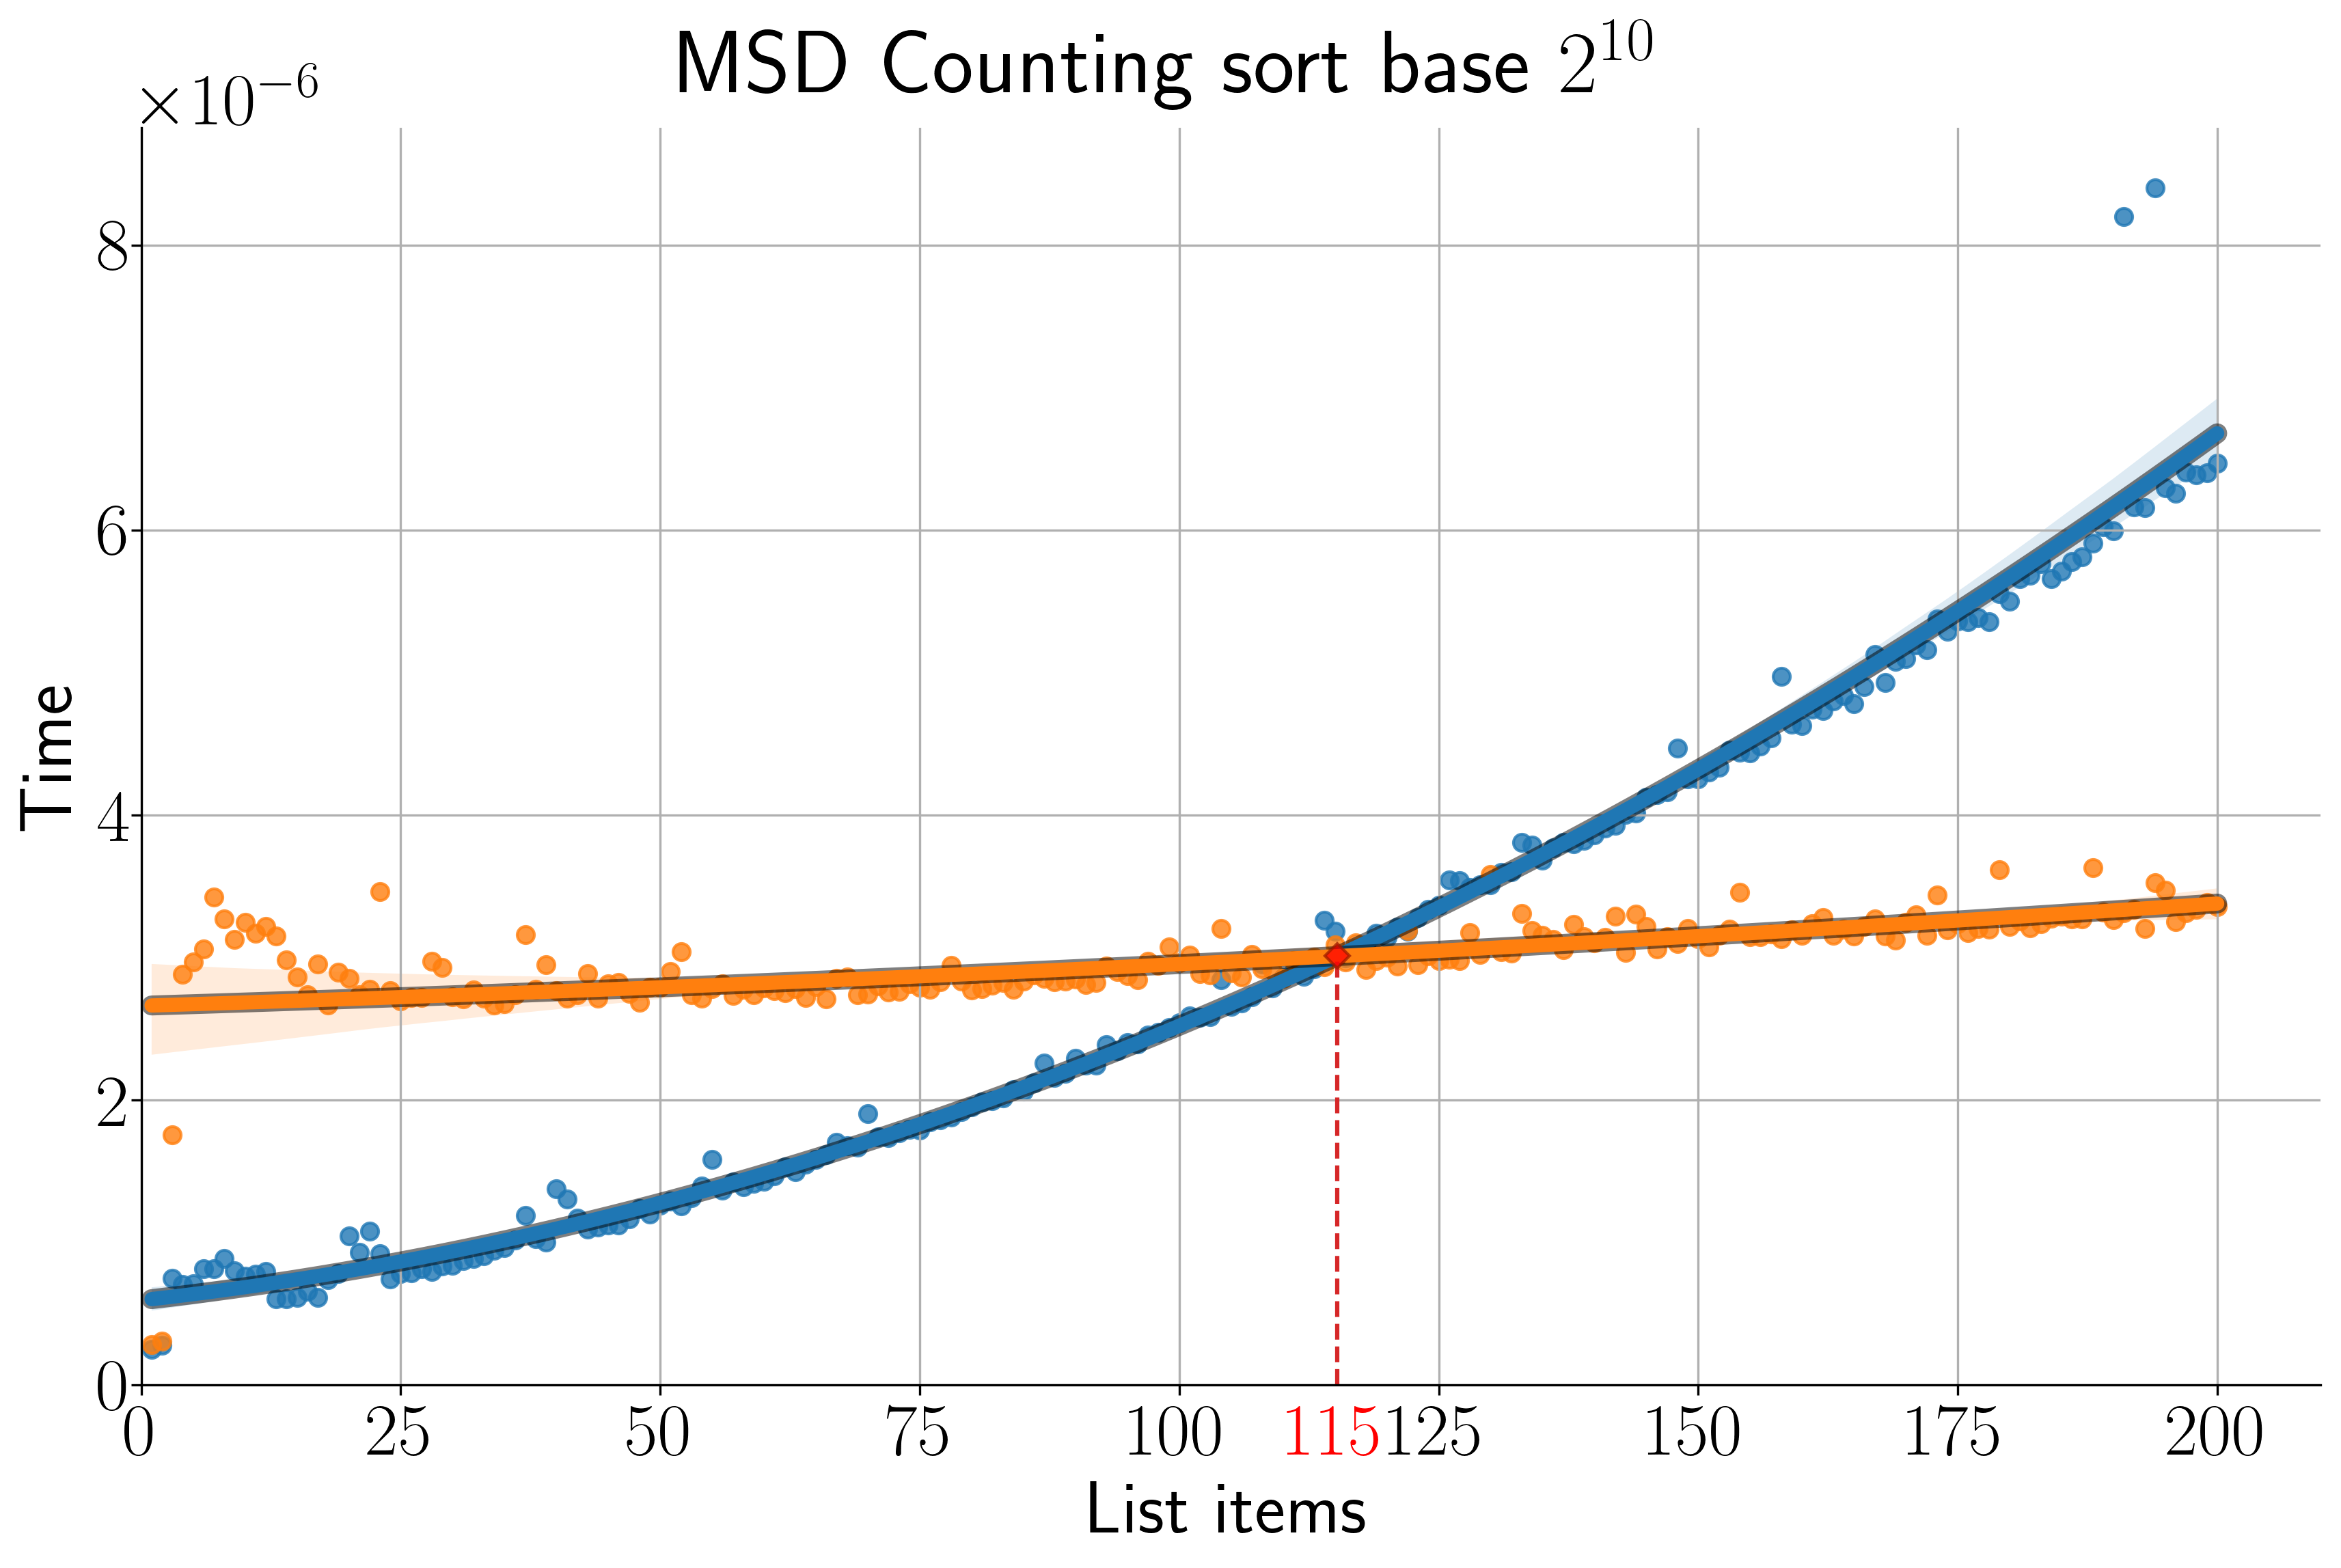
\includegraphics[width=.75\textwidth]{msd_c_10.png}}
		\raisebox{-0.5\height}{\includegraphics[width=.15\textwidth]{insertionLegend.png}}
		
		\captionof{figure}{Time comparison for insertion sort and radix sort using counting sort, base $2^{10}$}
		\label{fig:msdinsert}
	\end{minipage}
	
\end{table}
\pagebreak

\myparagraph{Profiling}
A tool Utilized to test the performance of solutions was a line profiler for Python, in this project the open source utility line\textunderscore profiler \cite{lineprof} was used. This tool runs a python script and returns information about executed code within a function, namely the execution time of each line per call, the number of calls of each line, the total number of times a line was called and the time taken by calling the line as a percentage of the total execution time of the script.
\par 
It is important to note that this tool runs using Python, not PyPy and also that as this project demands a compiled piece of code written in RPython the results regarding time taken must not be taken as too strongly indicative of the performance of a solution. It was also necessary to make minor changes to the code such as replacing \textit{xrange} with the equivalent \textit{range} and \textit{sys.maxint} with \textit{sys.maxsize}.
\par 
The data provided by this tool was, however, very useful at identifying the correctness of solutions as the number of calls to a particular line would be identical whether run using line\textunderscore profiler or with a compiled version of PyPy, provided the input list is identical. Using this information allowed me to ensure that the code was efficient and that unnecessary iterations over the input list were not made. As an example this tool allowed me to identify that pigeonhole sort was incorrectly performing an additional iteration by showing that all lists made up of positive integers triggered the condition of a single bucket containing all items.
\par
Initially one of the aims of testing was to complete a profile of the memory usage of the sort methods, however this was deemed to not be feasible as memory profiling in PyPy is highly inaccurate, and the function \textit{sys.getsizeof} is not included in PyPy causing an error for most memory profilers. According to the documentation, the reason for this is due to optimizations performed by the PyPy compiler that cause the size of most objects to be reported incorrectly, meaning any value returned by \textit{sys.getsizeof} would be meaningless \cite{pypymem}.

\begin{table}[H]
	\centering
	\makebox[\linewidth]{
	\resizebox{1.1\linewidth}{!}{
		\centering
	% \mbox{
	\begin{tabular}{rrrrrl}
		\hline
		Line \# & Hits   & Time   & Per Hit   & \% Time   & Line Contents                                                       \\
	 \hline
	 127 & 5     & 1.6    & 0.3    & 0.0  &  \;\;\;\;\lstinline{    for i in range(list_max_digits):}\\
	 128 & 4     & 1.6    & 0.4    & 0.0  &  \;\;\;\;\;\;\;\;\lstinline{        shift = (self.base) * i}\\
	 129 & 40004 & 4158.5 & 0.1    & 11.2 &  \;\;\;\;\;\;\;\;\lstinline{        for num in self.list:}\\
	 130 & 40000 & 6395.9 & 0.2    & 17.2 &  \;\;\;\;\;\;\;\;\;\;\;\;\lstinline{            masked_input = num ^ bit_mask}\\
	 131 & 40000 & 9121.8 & 0.2    & 24.5 &  \;\;\;\;\;\;\;\;\;\;\;\;\lstinline{            curr_digit = (masked_input >> shift) & self.radix - 1}\\
	 132 & 40000 & 8222.3 & 0.2    & 22.1 &  \;\;\;\;\;\;\;\;\;\;\;\;\lstinline{            bucket_list[curr_digit].append(num)}\\
	 133 & 8     & 117.4  & 14.7   & 0.3  &  \;\;\;\;\;\;\;\;\lstinline{        nonempty = [}\\
	 134 &       &        &        &      &  \;\;\;\;\;\;\;\;\;\;\;\;\lstinline{            (bdx, bucket)}\\
	 135 & 4     & 6.1    & 1.5    & 0.0  &  \;\;\;\;\;\;\;\;\;\;\;\;\lstinline{            for bdx, bucket in enumerate(bucket_list)}\\
	 136 &       &        &        &      &  \;\;\;\;\;\;\;\;\;\;\;\;\lstinline{            if bucket != []}\\
	 137 &       &        &        &      &  \;\;\;\;\;\;\;\;\lstinline{        ]}\\
	 138 & 4     & 3.6    & 0.9    & 0.0  &  \;\;\;\;\;\;\;\;\lstinline{        if len(nonempty) == 1:}\\
	 139 &       &        &        &      &  \;\;\;\;\;\;\;\;\;\;\;\;\lstinline{            bucket_list[nonempty[0][0]] = []}\\
	 140 &       &        &        &      &  \;\;\;\;\;\;\;\;\;\;\;\;\lstinline{            continue}\\
	 141 & 4     & 1.0    & 0.3    & 0.0  &  \;\;\;\;\;\;\;\;\lstinline{        index = 0}\\
	 142 & 260   & 37.6   & 0.1    & 0.1  &  \;\;\;\;\;\;\;\;\lstinline{        for bdx, bucket in enumerate(bucket_list):}\\
	 143 & 256   & 41.8   & 0.2    & 0.1  &  \;\;\;\;\;\;\;\;\;\;\;\;\lstinline{            if len(bucket) == 0: continue}\\
	 144 & 200   & 257.8  & 1.3    & 0.7  &  \;\;\;\;\;\;\;\;\;\;\;\;\lstinline{            self.setslice(bucket, index)}\\
	 145 & 200   & 36.1   & 0.2    & 0.1  &  \;\;\;\;\;\;\;\;\;\;\;\;\lstinline{            index += len(bucket)}\\
	 146 & 200   & 37.1   & 0.2    & 0.1  &  \;\;\;\;\;\;\;\;\;\;\;\;\lstinline{            bucket_list[bdx] = []}\\
	 \hline
		\end{tabular}
		}}
		\caption*{excerpt from line\textunderscore profiler output of LSD Counting sort}
	\end{table}
\pagebreak
\myparagraph{Order checking}
\label{sssec:orderchecking}
As an extension of the sort check made at the start of each call to radix sort, in MSD sort, it is possible to check sub lists for being sorted or reverse sorted after each iteration of integer sorting to identify lists that can be excluded from sorting on subsequent digits. Whether or not this strategy is effective is a trade off between the time saved from reduced iterations of integer sorting versus the time taken to complete this check. There is no similar optimization for LSD sorts as the list is never broken down into sub lists and so the entire list must be checked for randomly becoming sorted which is such a rare occurrence that it is not worth considering.
\par
\begin{lstlisting}	
	def slice_sorted(self, start=0, end=-1):
		end = end if end > -1 else self.list_length
		assert start >= 0
		assert end >= 0
		sub list_sorted, sub list_reverse_sorted = True, True
		for i, el in enumerate(self.list[start + 1 : end]):
			if el < self.list[start + i]:
				sub list_sorted = False
				if sub list_reverse_sorted == False:
					return sub list_sorted, sub list_reverse_sorted
			if el > self.list[start + i]:
				sub list_reverse_sorted = False
				if sub list_sorted == False:
					return sub list_sorted, sub list_reverse_sorted
		return sub list_sorted, sub list_reverse_sorted
\end{lstlisting}
\par
To evaluate the effectiveness of order checking, two versions of PyPy were compiled, one with the above function being used on every sub list and one without. These were then tested on lists of $1$,$000$,$000$ on lists containing random, nearly sorted and few unique data. The results of the tests showed that in almost all cases the order checking has a detrimental or limited positive effect and therefore this function was not included in this project. The figure below shows two examples of these tests and are representative of the other results.

\begin{table}[h]
	\centering
	\makebox[\linewidth]{
	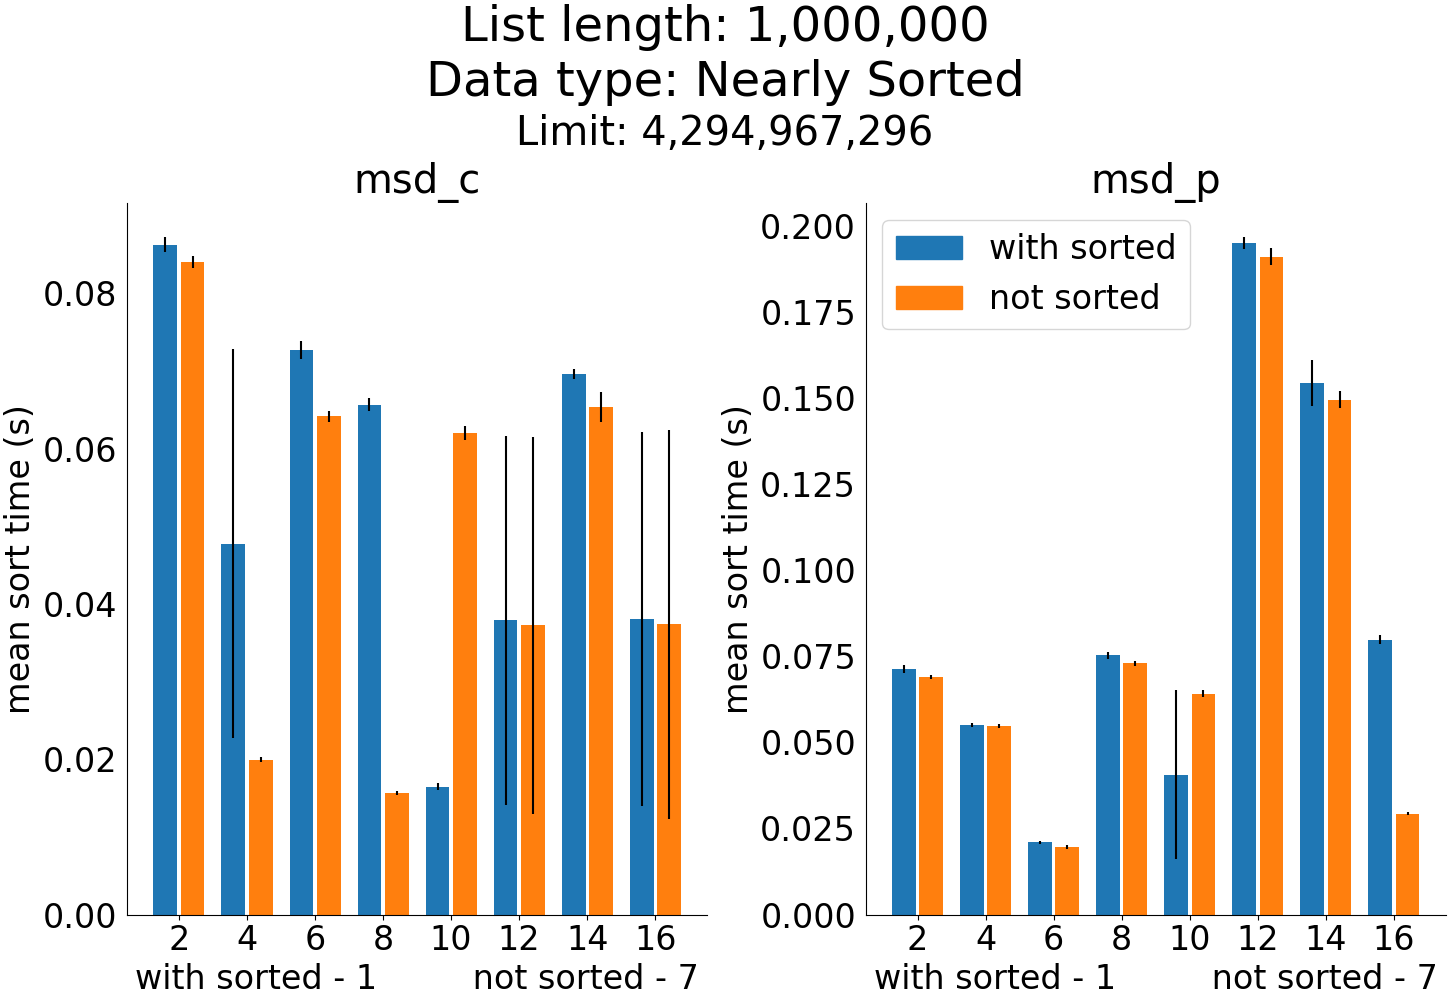
\includegraphics[ draft=false, height=5.5cm]{lrg_Nearly_Sorted_sorted_1.png}
	\hspace{0.25cm}
	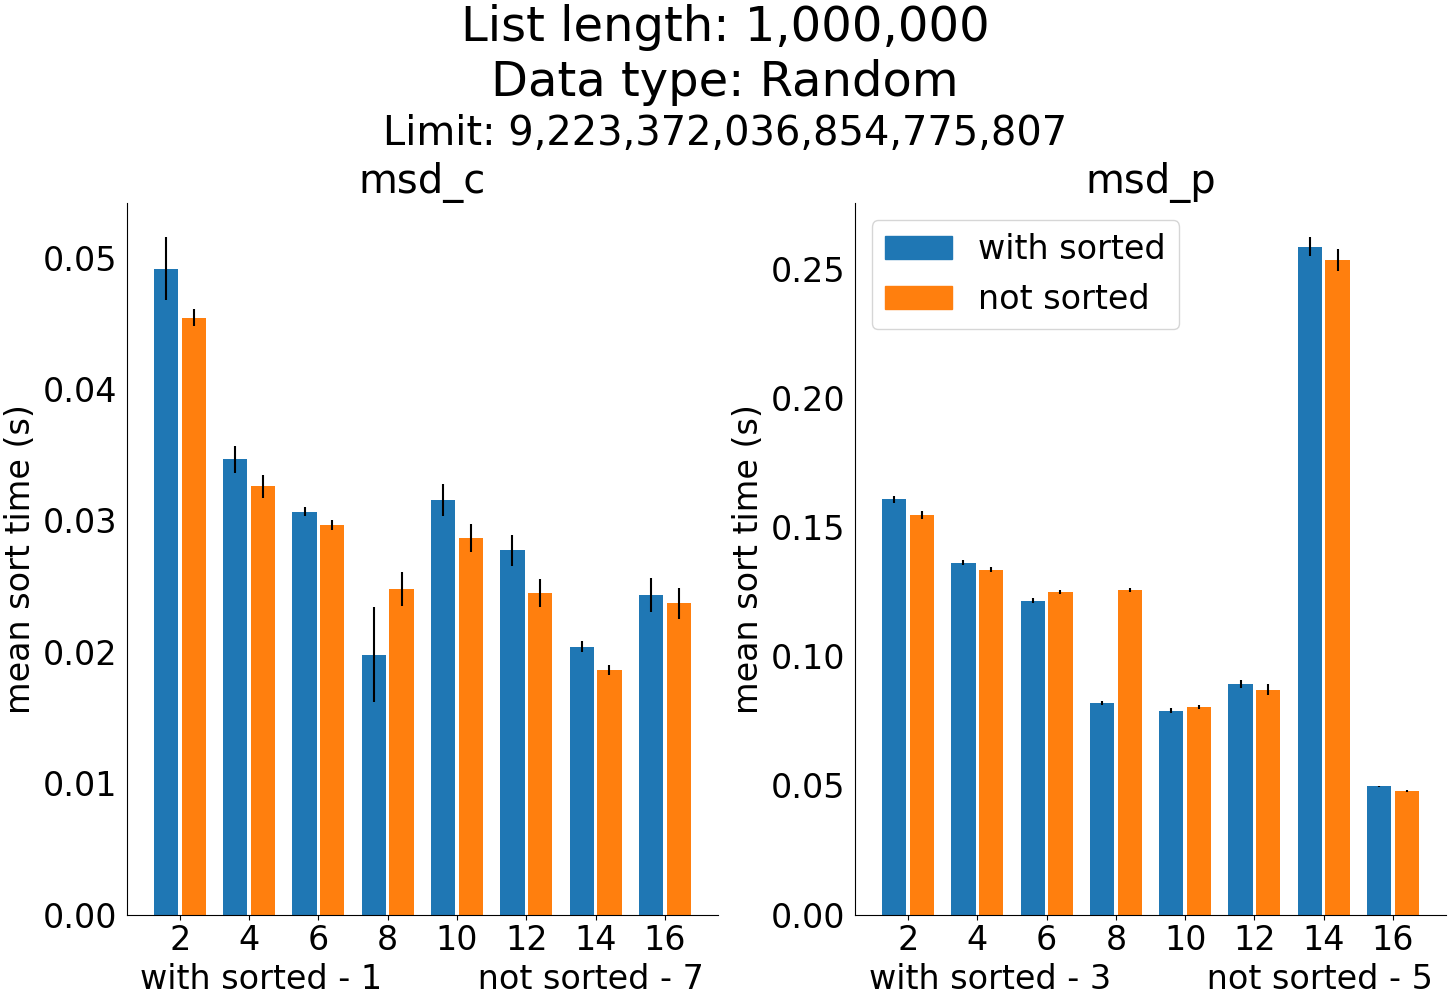
\includegraphics[ draft=false, height=5.5cm]{lrg_Random_sorted_0.png}
	}
	\captionof{figure}{The effects of completing order checking across sub lists. Listed below are the number of bases for which sort checking and not checking are the fastest option}
	
\end{table}

	\pagebreak
	\subsubsection{Test criteria}
	The purpose of the testing was primarily to compare the efficacy of the solution in this project to Timsort and verify whether the project goal of producing a more optimal sort method had been achieved. Secondary goals of the tests were to identify which of the 4 solutions performs the best and which base as the most effective as well as apply the algorithms to a variety of lists to identify the situations in which the algorithms were strong or weak relative to one another and to Timsort.
	\par
	As outlined in \ref{ssec:timecomplexity}, Radix sort has a time complexity that depends on the list length $n$ and the number of digits $d$, therefore a complete testing must evaluate the effect of these two variables on the run time of the algorithms. Measuring the effect of altering $n$ and $d$ was performed in two separate ways, in the first each was isolated and tested as a continuous variable without altering the other, in the second $3$ values were chosen for $n$ as well as $4$ ranges for list item values that contain different amounts of digits to test $d$. 
	\par
	The continuous testing of $n$ involved generating lists with a value for $n$ in the range $[1..1$,$000$,$000]$ and with list values of up to the maximum value for integers to ensure as best as possible that $d$ was constant. To test $d$, lists were generated with values constrained to the range $[-2^b..2^b\minus1]$ where $b$ varies from $[1..63]$, thereby increasing the value of $d$ but keeping $n$ constant.
	\par
	The non-continuous testing evaluated the run time of the algorithms of lists with a length of $10$,$000$, $100$,$000$ and $1$,$000$,$000$ and containing items with values within the range $[-2^{r}$ $..$ $2^{r}\minus1]$ where $r$ is $16$, $20$, $32$ and $63$. These parameters were selected to provide tests that represent the smallest and largest extremes of the continuous tests as well as some tests in the middle. 
	\par
	Testing had to be split into continuous and non-continuous as performing a continuous evaluation of both $n$ and $d$ would require a test of all values of $d$ performed for all values of $n$ and the amount of tests necessary makes this unfeasible. Furthermore, the data created by this would span 3 dimensions and would be difficult to extract useful information from. The continuous tests are useful for identifying the differences between each numerical base used for the algorithms, but as they are primarily evaluating the effect of $n$ and $d$ on Radix sort, they are not suitable for making a comparison to Timsort, the sort method used in \textit{listsort.py}.
	\par
	As the non-continuous testing evaluates a range of both $n$ and $d$, the non-continuous testing is also performed on lists generated in different format to evaluate each algorithms performance in the widest range of circumstances. The formats used are identified in \ref{sssec:methodology} (Random, Nearly sorted and Few Unique). This type of testing was used to make a final comparison to Timsort, which is optimized for efficiency on lists with sorted sub-sections and therefore highly performant on nearly sorted lists.
	\par
	\pagebreak
	\subsection{Test results and analysis} 
	\subsubsection{Varying list length}
	This test shows the effect of list size on the performance of radix sort and very clearly highlights the difference between the bases used. Some bases produce results that stretch the size of the graph so much that it prevents meaningful information from being shown, hence some graphs have non-competitive bases omitted for readability.
	\par To prevent the focus of this analysis being unfairly weighted towards lists of lengths closer to $1$,$000$,$000$ where the difference between run times is larger and therefore more visible on graphs, where the results may be different to lower list length, and which may not represent the most common use case for this algorithm, these tests were also performed with lists of length $100$,$000$. 
	\myparagraph{LSD Counting sort}
	The results show that at all small list lengths, sort times are comparable but above lengths of $65$,$536$ bases $8$ ad $16$, which were slightly faster, become slower and do not recover at any point up to $1$,$000$,$000$. This critical value likely exists at this point as it is $2^{16}$ and as 16 is divisible by both values and therefore is the point where another digit is needed for sorting, but all other bases also take slight jumps at this stage and this is the most pronounced increase on either graph which indicates there may be some sort of cache limitation at this value (similar to what is discussed in \ref{ssec:radixexplanation}), alternatively, PyPy may be optimizing the storage of lists into chunks of this size.

	\par
	Base $6$ is the slowest shown, performing similarly to 8 and 16 around 100,000 items but falls off as more items are added. This bases seem to be too small to be suitable for this type of radix sort and this result is compounded in the omitted bases 4 and 2 which was the worse performer.
	\par
	Overall, the results show $10$ is the best performing base here, but it is only narrowly better than the $12$ and $14$ which are slightly faster than bases $8$ and $16$ with 6 showing a clear deficit particularly at greater list lengths.

	\begin{table}[h]
		\centering
		\makebox[\linewidth]{
			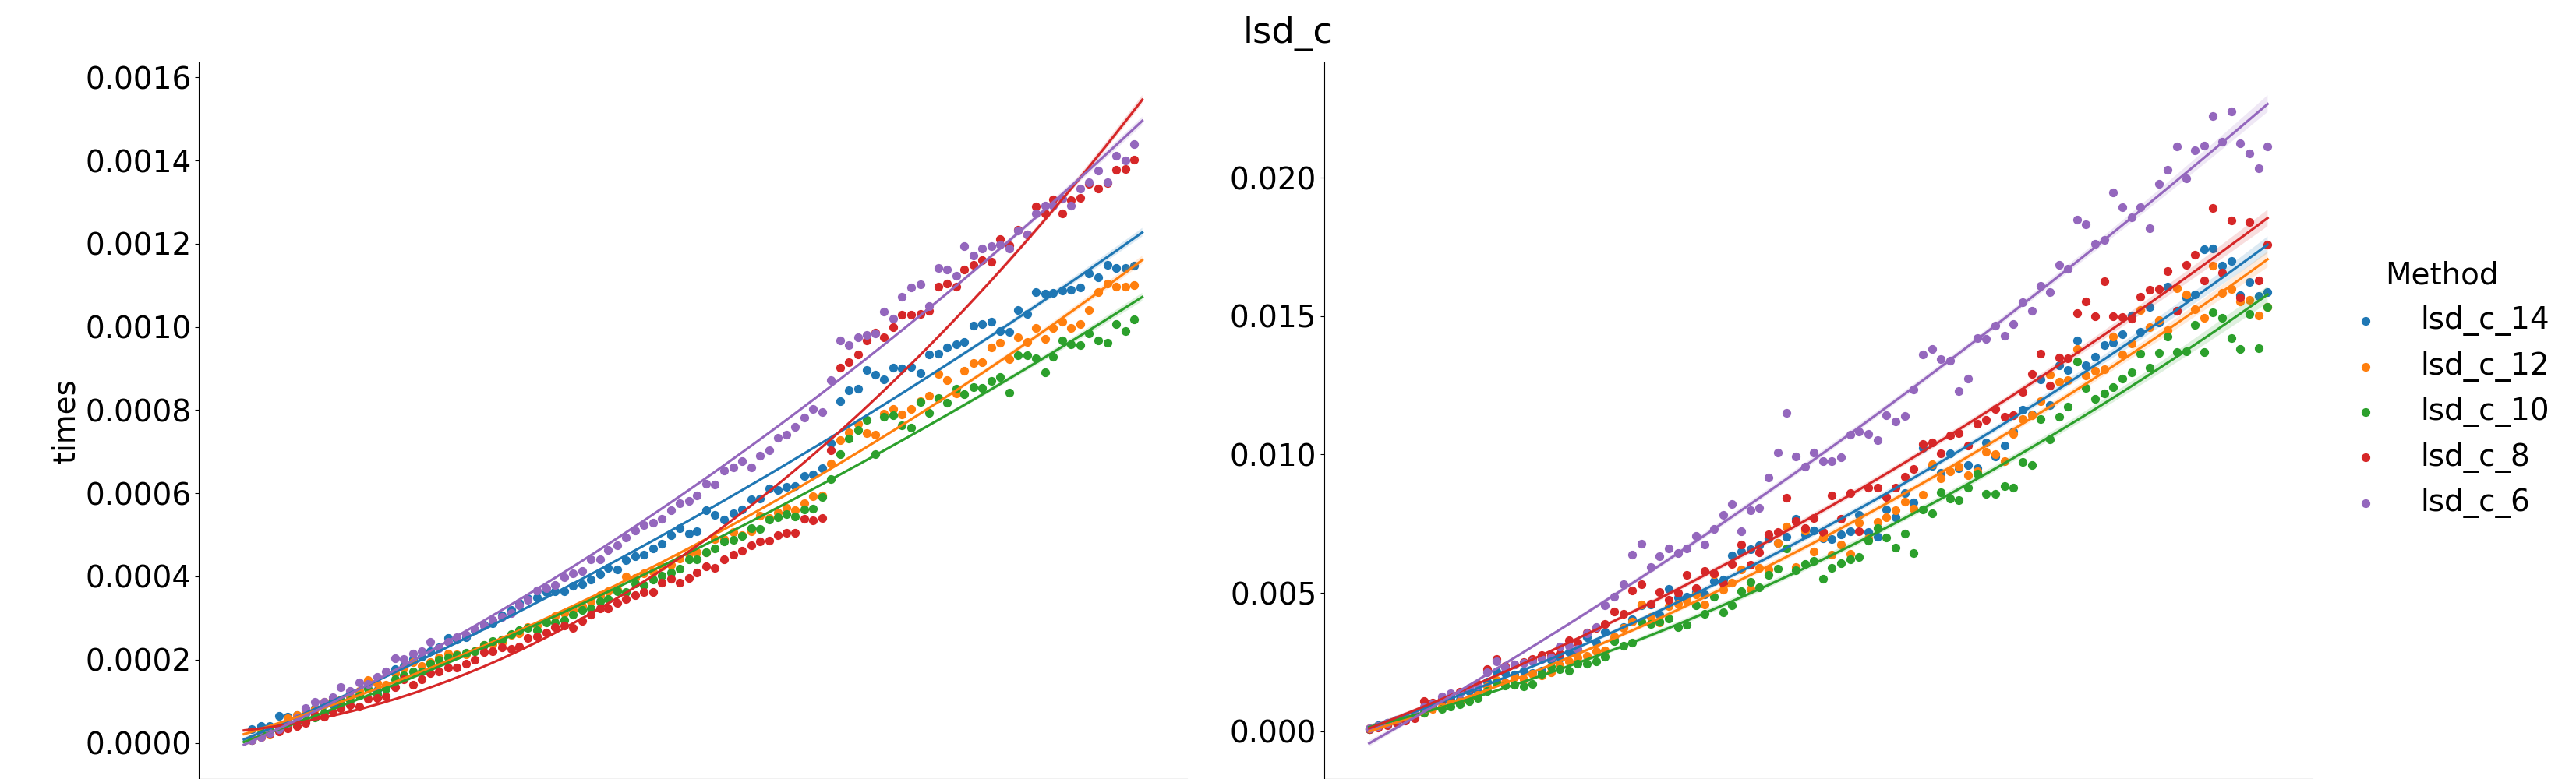
\includegraphics[ draft=false,width=1.1\linewidth]{lsd_c_length}
			}
			\caption*{LSD Counting sort length test for 100,000 and 1,000,000 items \par bases 2, 4, 6 and 8 omitted}
	\end{table}
	\pagebreak

	\myparagraph{LSD Pigeonhole sort}
	The fastest base for LSD Pigeonhole varies a lot among the best performers as list length increases. Bases 16, 14, 12 and 10 appear intertwined from 200,000 to 1,000,000 items with 16 ahead at the 1,000,000 point but not by a large margin. Bases 8 and below are omitted from the 1,000,000 graph as they are notably slower in this range.
	\par
	Though base 16 becomes the most effective at higher list lengths, it is not truthful to call it the best as it is nearly 10 times slower than base $10$ for list lengths below $100$,$000$. For this reason bases 10 and 12 would be the most suitable, as base 14 is also noticeably slower for lower lengths, albeit less pronounced than 16.
	\begin{table}[h]
		\centering
		\makebox[\linewidth]{
			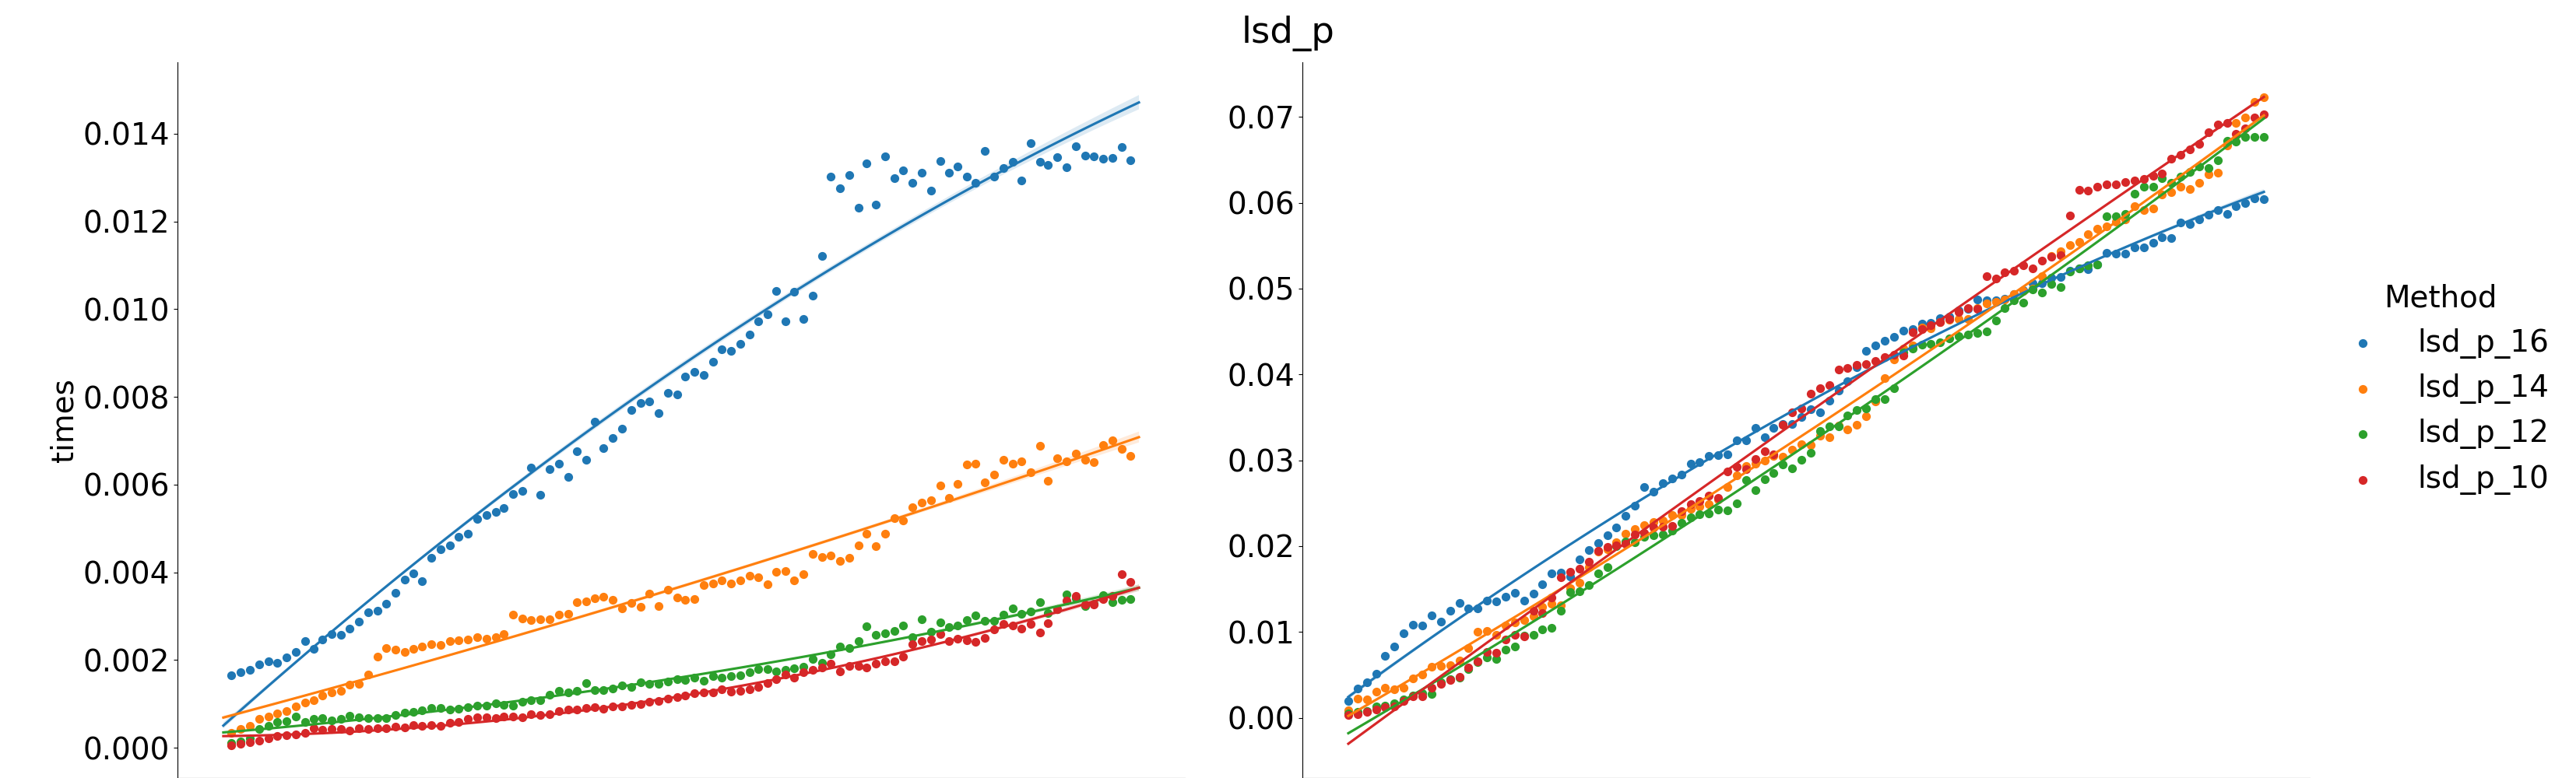
\includegraphics[ draft=false,width=1.1\linewidth]{lsd_p_length}
			}
			\caption*{LSD Pigeonhole sort length test for 100,000 and 1,000,000 items \par bases 2 and 4 omitted}
	\end{table}
	\myparagraph{MSD Counting sort}
	The results visible here are highly similar to those of LSD counting sort, base 6 becomes more performant than 8 and 16 in the lower range, but again lags behind in the higher range. Once again, base 10 performs best with similar grouping of the other bases.
	\begin{table}[h]
		\centering
		\makebox[\linewidth]{
			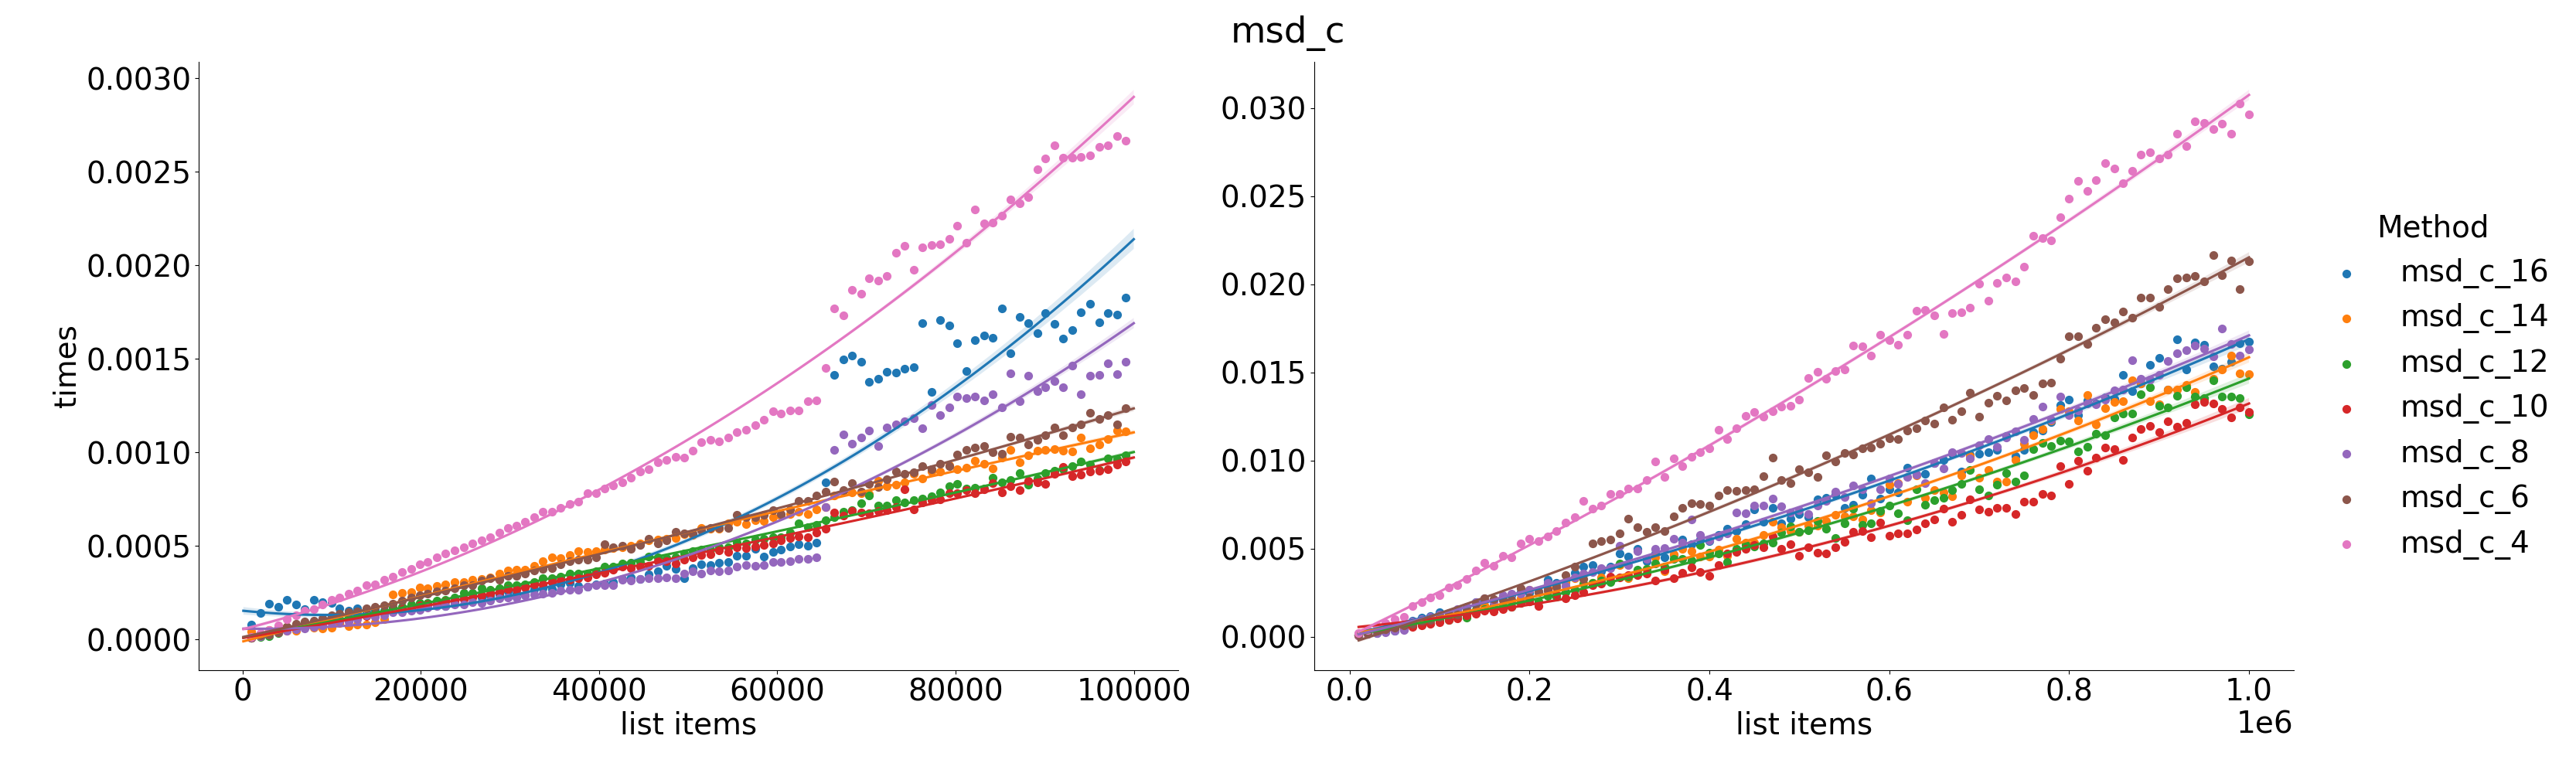
\includegraphics[ draft=false,width=1.1\linewidth]{msd_c_length}
			}
			\caption*{MSD Counting sort length test for 100,000 and 1,000,000 items \par base 2 omitted}
	\end{table}
	\pagebreak
	\myparagraph{MSD Pigeonhole sort}
	This set of results deviates significantly from the rest of this set, it shows that the larger bases are unsuitable for this implementation, with base 16 being the worst. This is the only iteration of this test in which base 2 wasn't the worst performer.
	\par
	The ideal range appears to be around base 6, with 4 and 8 roughly equivalent in performance, as are 2 and 10, above which a base increase is detrimental.
	\vspace{-0.5cm}
	\begin{table}[h]
		\centering
		\makebox[\linewidth]{
			\setlength{\floatsep}{0pt}
			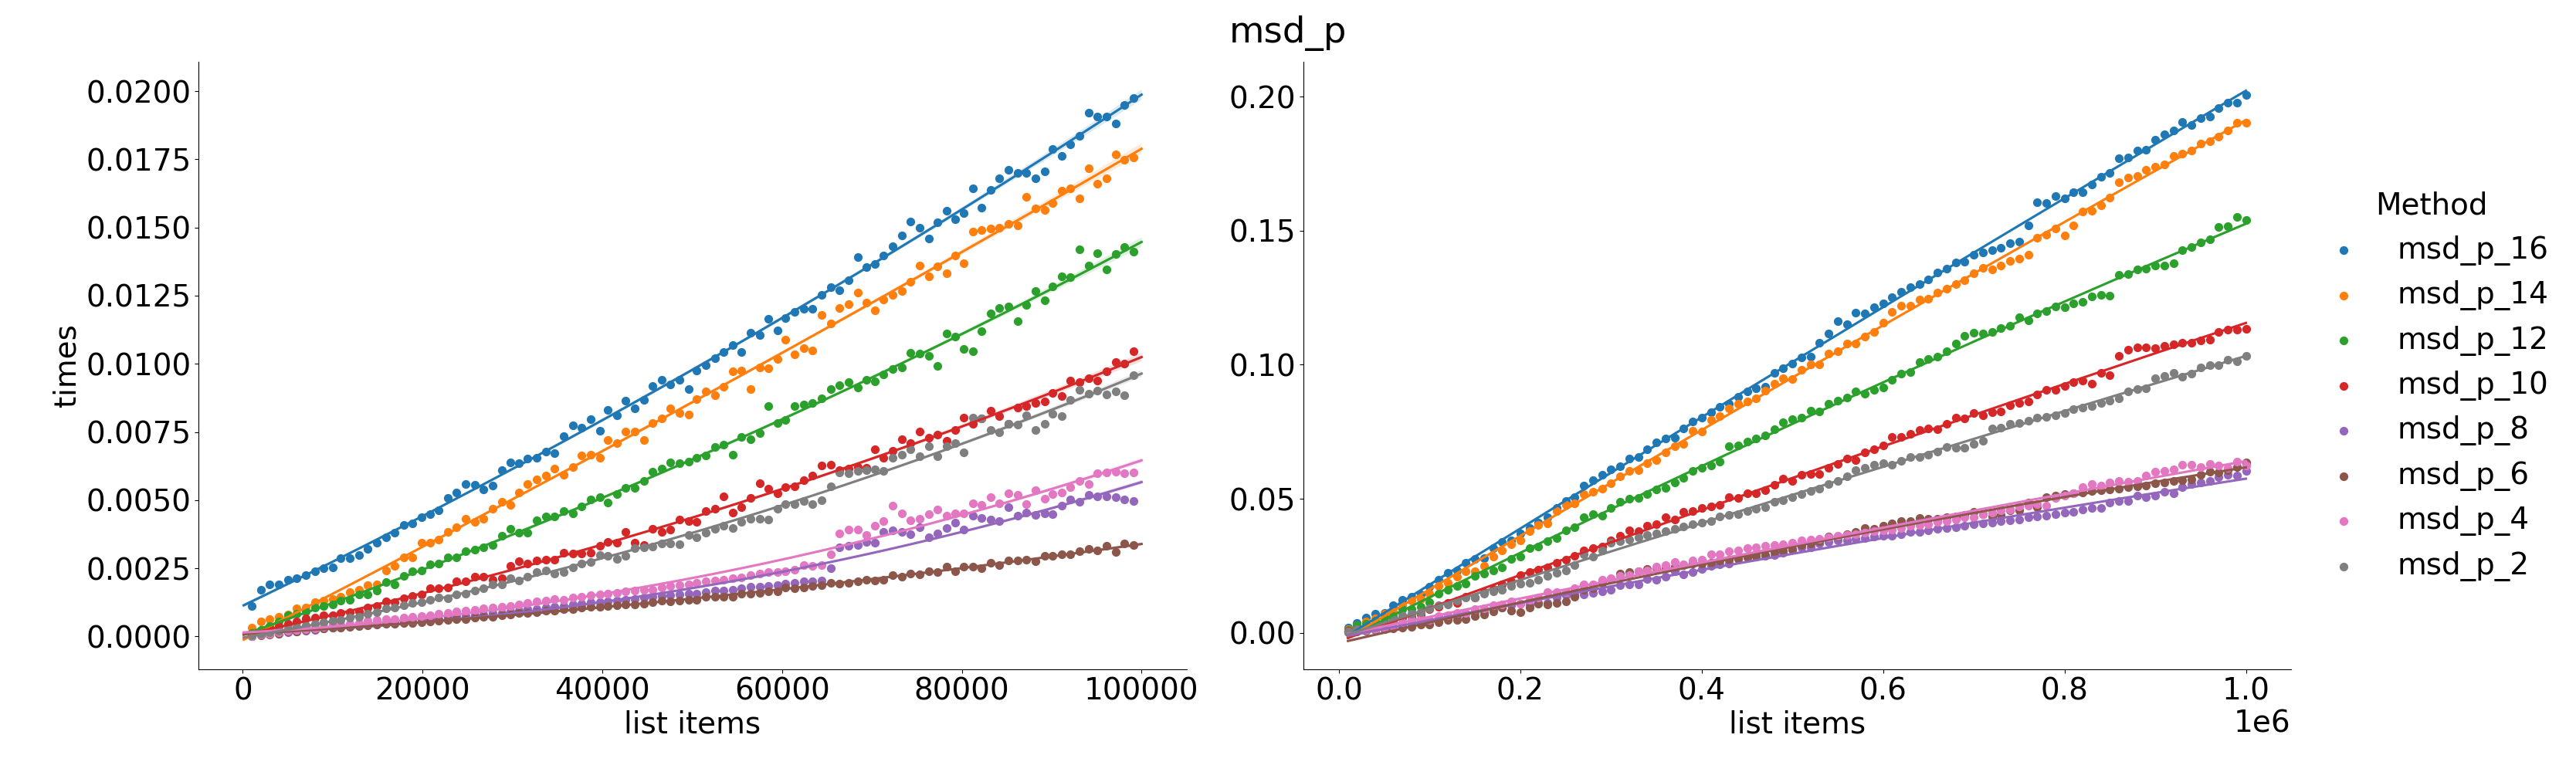
\includegraphics[ draft=false,width=1.1\linewidth]{msd_p_length}
			}
			\caption*{MSD pigeonhole sort length test}	
	\end{table}
	\vspace{-1cm}
	\subsubsection{Varying base}
	This test examines lists of 1,000,000 items generated randomly within the range $[\minus2^r..2^r\minus1]$ where r is the $data$\textunderscore $size$ referenced on the x axis. It is designed to test the algorithm's response to an increasing number of digits.
	\par
	This test is limited when applied to MSD radix sorts due to the algorithms ability to terminate sorting on smaller lists via insertion sort or sorting a list into a sub list of length 1, this means that typically a list of 1,000,000 items is sorted when $20/{base}$ digits have been sorted as $2^{20}$ is the smallest power of 2 greater than the list length. This is visible in the results as the sort times level out after $data$\textunderscore $size$ and does restrict the usefulness of the results but does present an interesting benefit of MSD sorting.
	\myparagraph{LSD Counting}
	The results shown on this graph are so similar that any difference between them was completely unreadable if any of the other bases were not omitted, showing that any of the bases 8,10,12,16 are suitable. As is typical for this type of testing, the jump in run time as $data$\textunderscore $size$ reaches values divisible by each base is easily identifiable, showing the effect of each additional digit.
	\begin{table}[h]
		\centering
		\makebox[\linewidth]{
			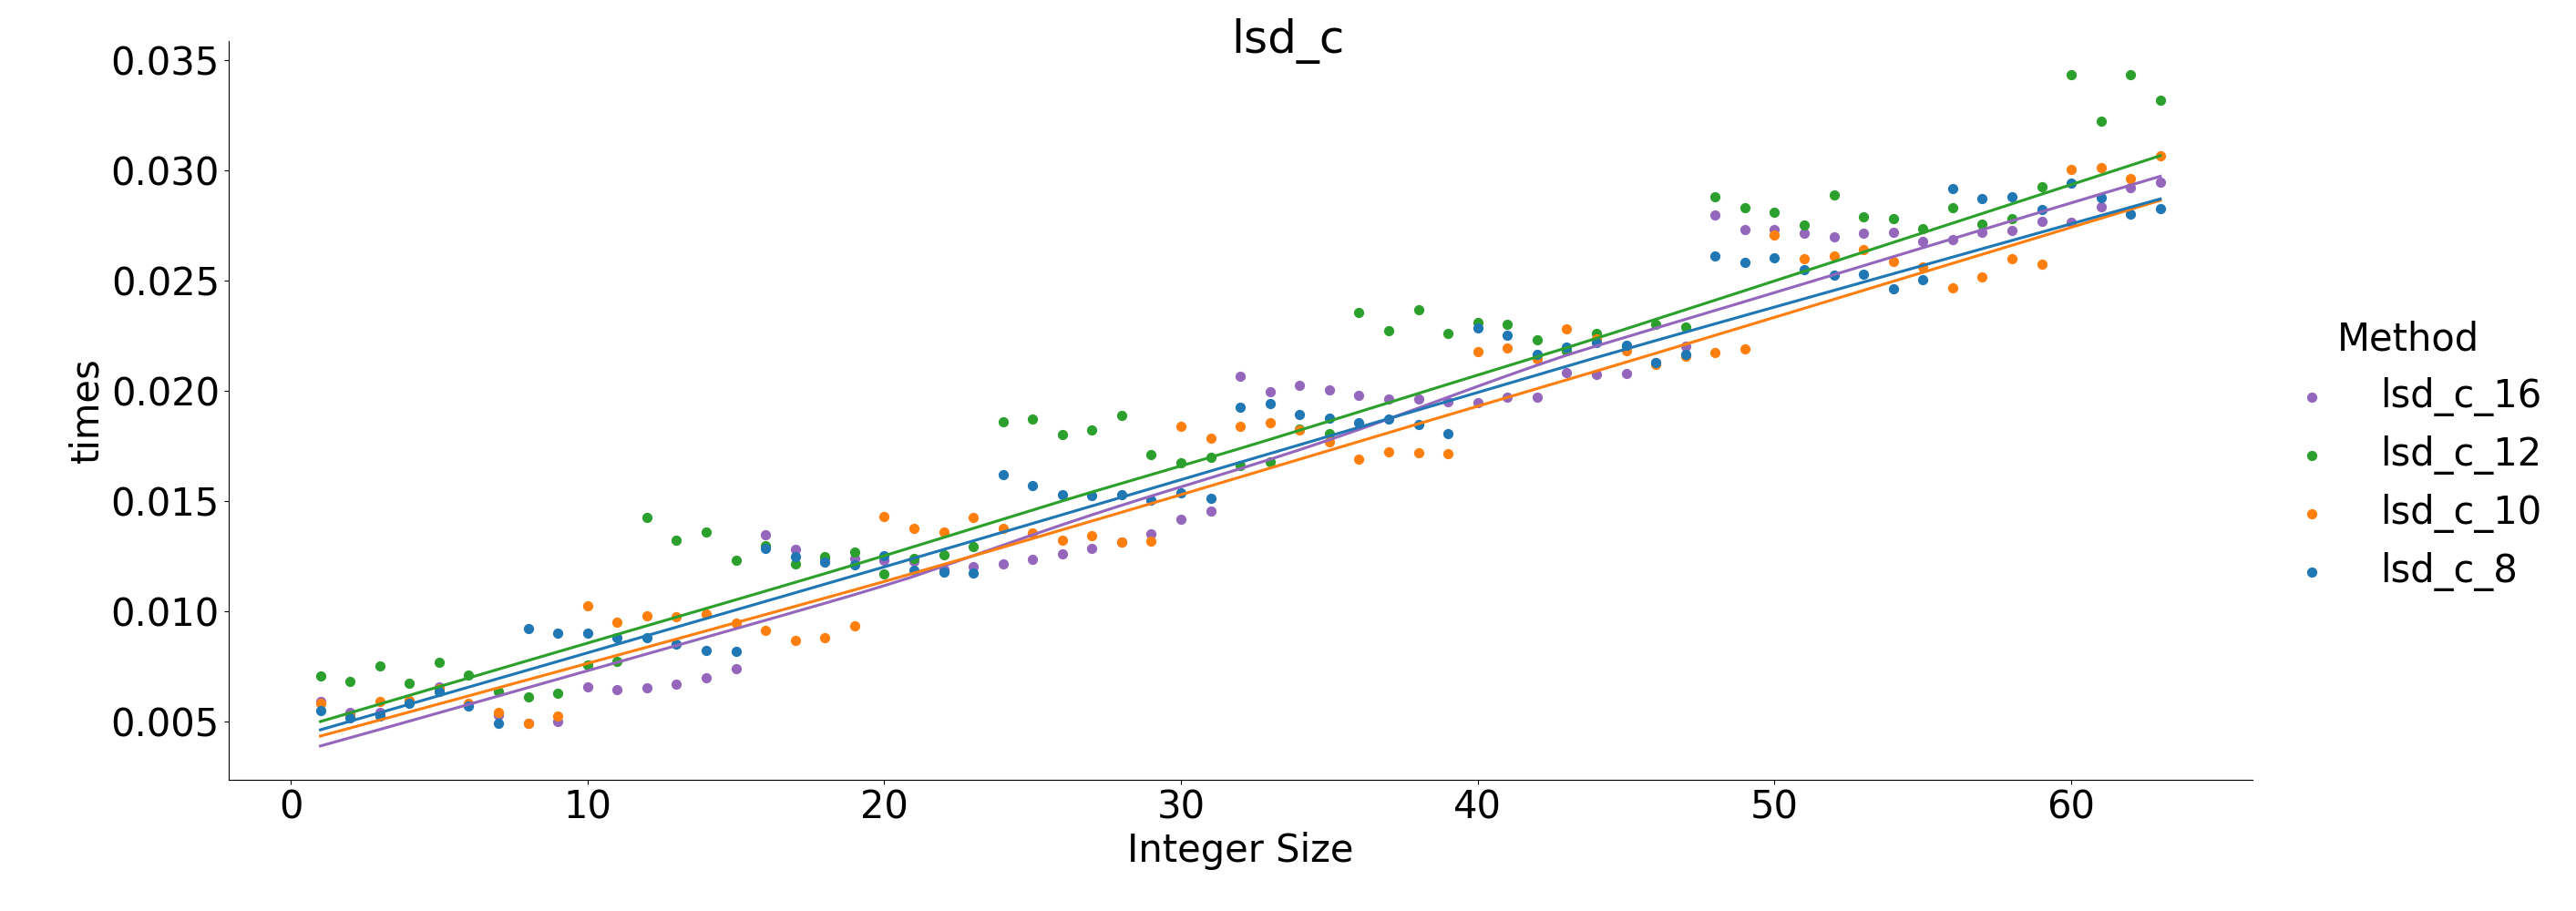
\includegraphics[ draft=false,height=4.8cm]{lsd_c_base}
		}
			\caption*{LSD counting sort input limit test}
	\end{table}
	\vspace{-1cm}
	\myparagraph{LSD Pigeonhole}
	The results for LSD Pigeonhole sort show higher bases performing better than lower bases, with 16 and 14 performing the best and almost identically which indicates that the results for the list length results for base 14 (in which it was slower than base 12 and 10 at 1,000,000 items) may be anomalous.
	\begin{table}[h]
		\centering
		\makebox[\linewidth]{
			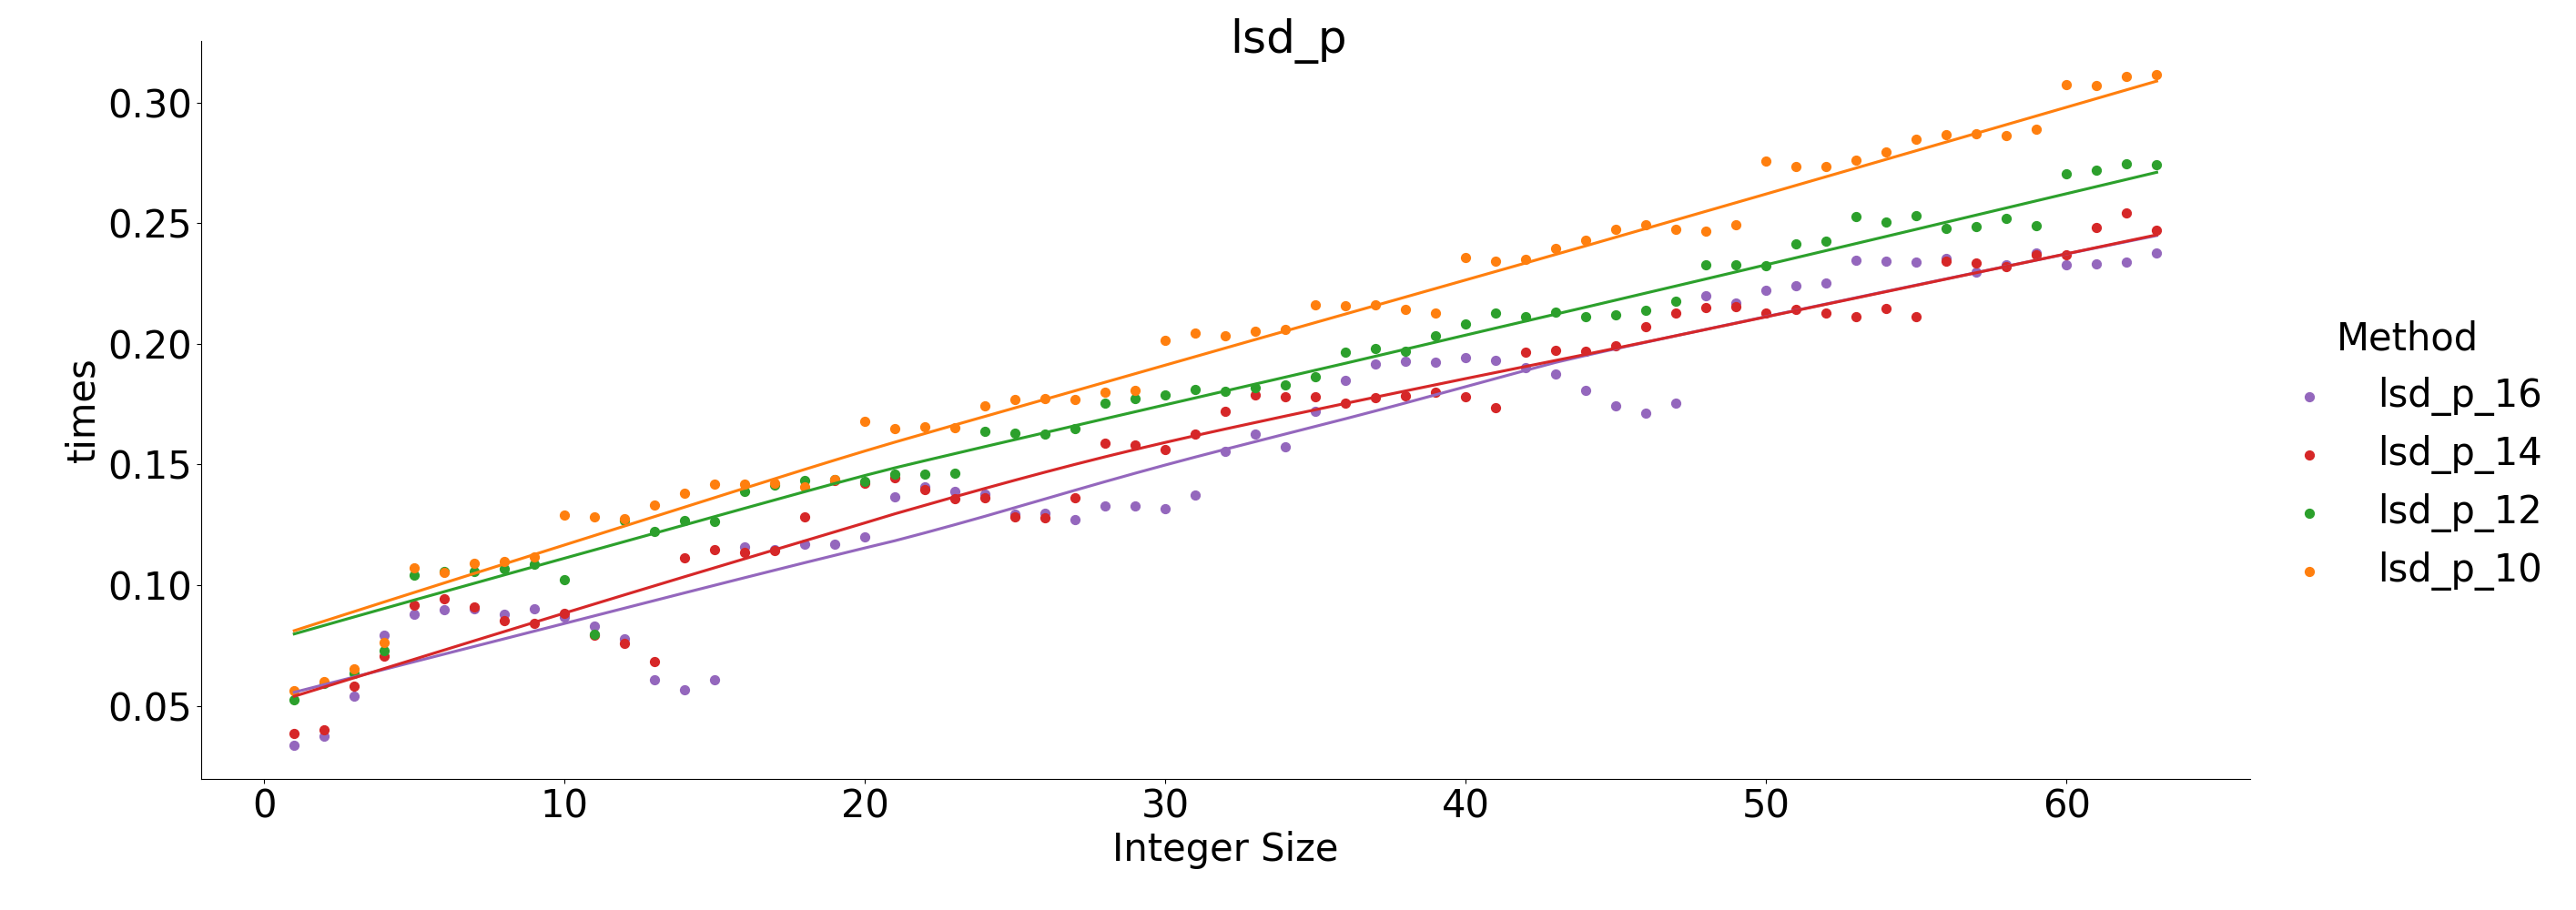
\includegraphics[ draft=false,height=4.8cm]{lsd_p_base}
		}
			\caption*{LSD pigeonhole sort input limit test}
	\end{table}
	\myparagraph{MSD Counting}
	As already stated, the usefulness of results of this type of test for this algorithm is limited, but of the most performant algorithms, 10 and 12 , the results for base 10 show a smaller delta between the maximum and minimum times with very similar times overall
	\begin{table}[h]
		\centering
		\makebox[\linewidth]{
			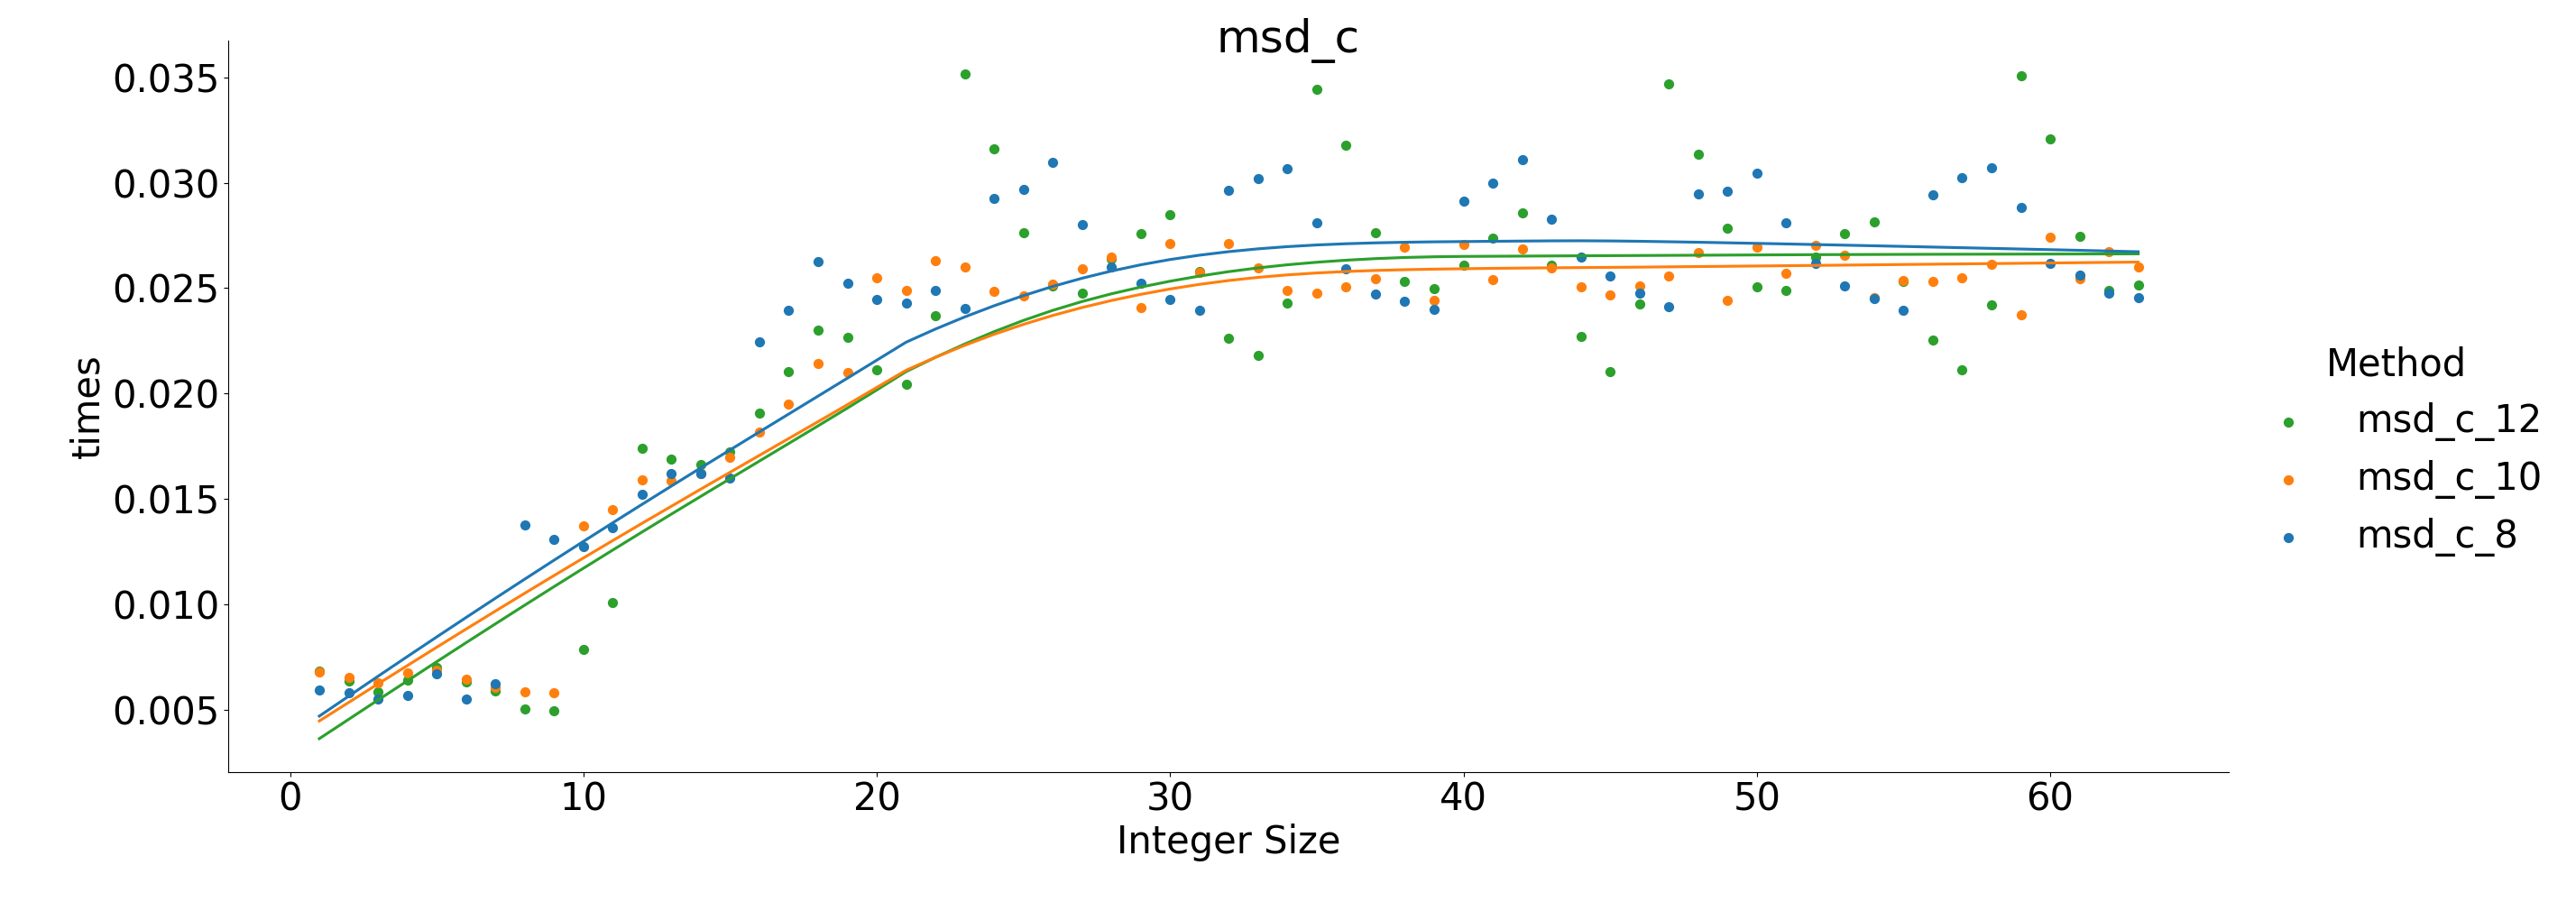
\includegraphics[ draft=false,height=4.8cm]{msd_c_base}
		}
			\caption*{MSD counting sort input limit test}
	\end{table}
	\pagebreak
	\myparagraph{MSD Pigeonhole}
	MSD pigeonhole again has results quite dissimilar from the other algorithms, the increase $data$\textunderscore $size$ has the smallest effect on the growth of run time and as the increases causes an additional digit's worth of sorting, the jump in run time is followed by a huge spike before falling again all in the range of values fitting onto the same digit. Drawing conclusions about any of these algorithms based on this data is almost impossible, but there isn't anything immediately wrong with bases 8 or 10, where base 8 is slightly slower but has smaller spikes in run time.
	\begin{table}[h]
		\centering
		\makebox[\linewidth]{
			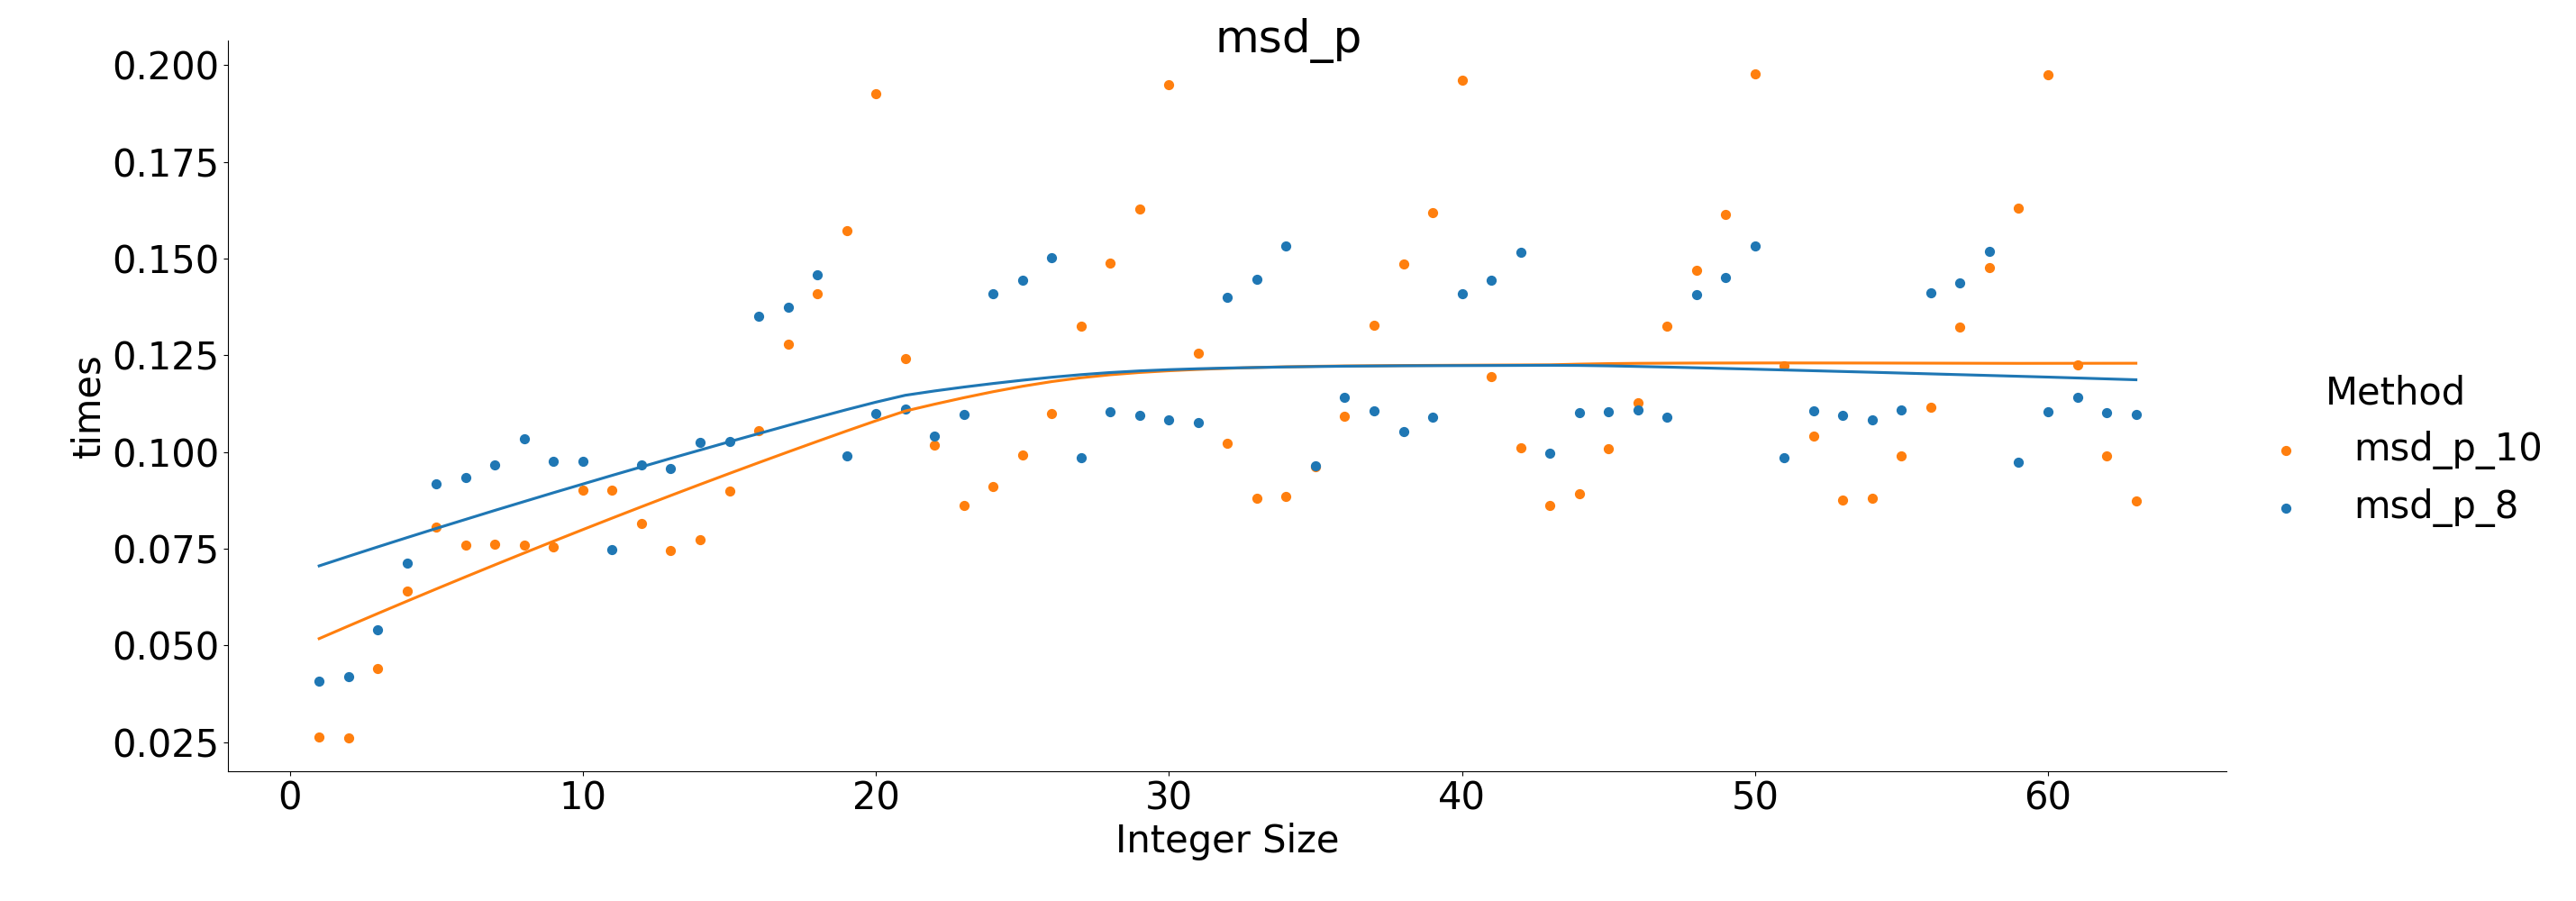
\includegraphics[ draft=false,height=4.8cm]{msd_p_base}
		}
			\caption*{MSD pigeonhole sort input limit test}
	\end{table}
	\subsubsection{Categorical tests}
	These tests were completed to provide an opportunity to make comparisons between the 4 algorithms, the 8 bases used and give insight into their effectiveness relative to Timsort. Each image shows the results for a list length and data type identified in the title, a set of axes for each data size listed as a subtitle and on each axis is the 4 algorithms developed for this project split into a bar for each base alongside timsort farthest on the right which has a line stretching across the axis to aid comparison to each implementation.
	\begin{table}[b]
		\centering
		\makebox[\linewidth]{
			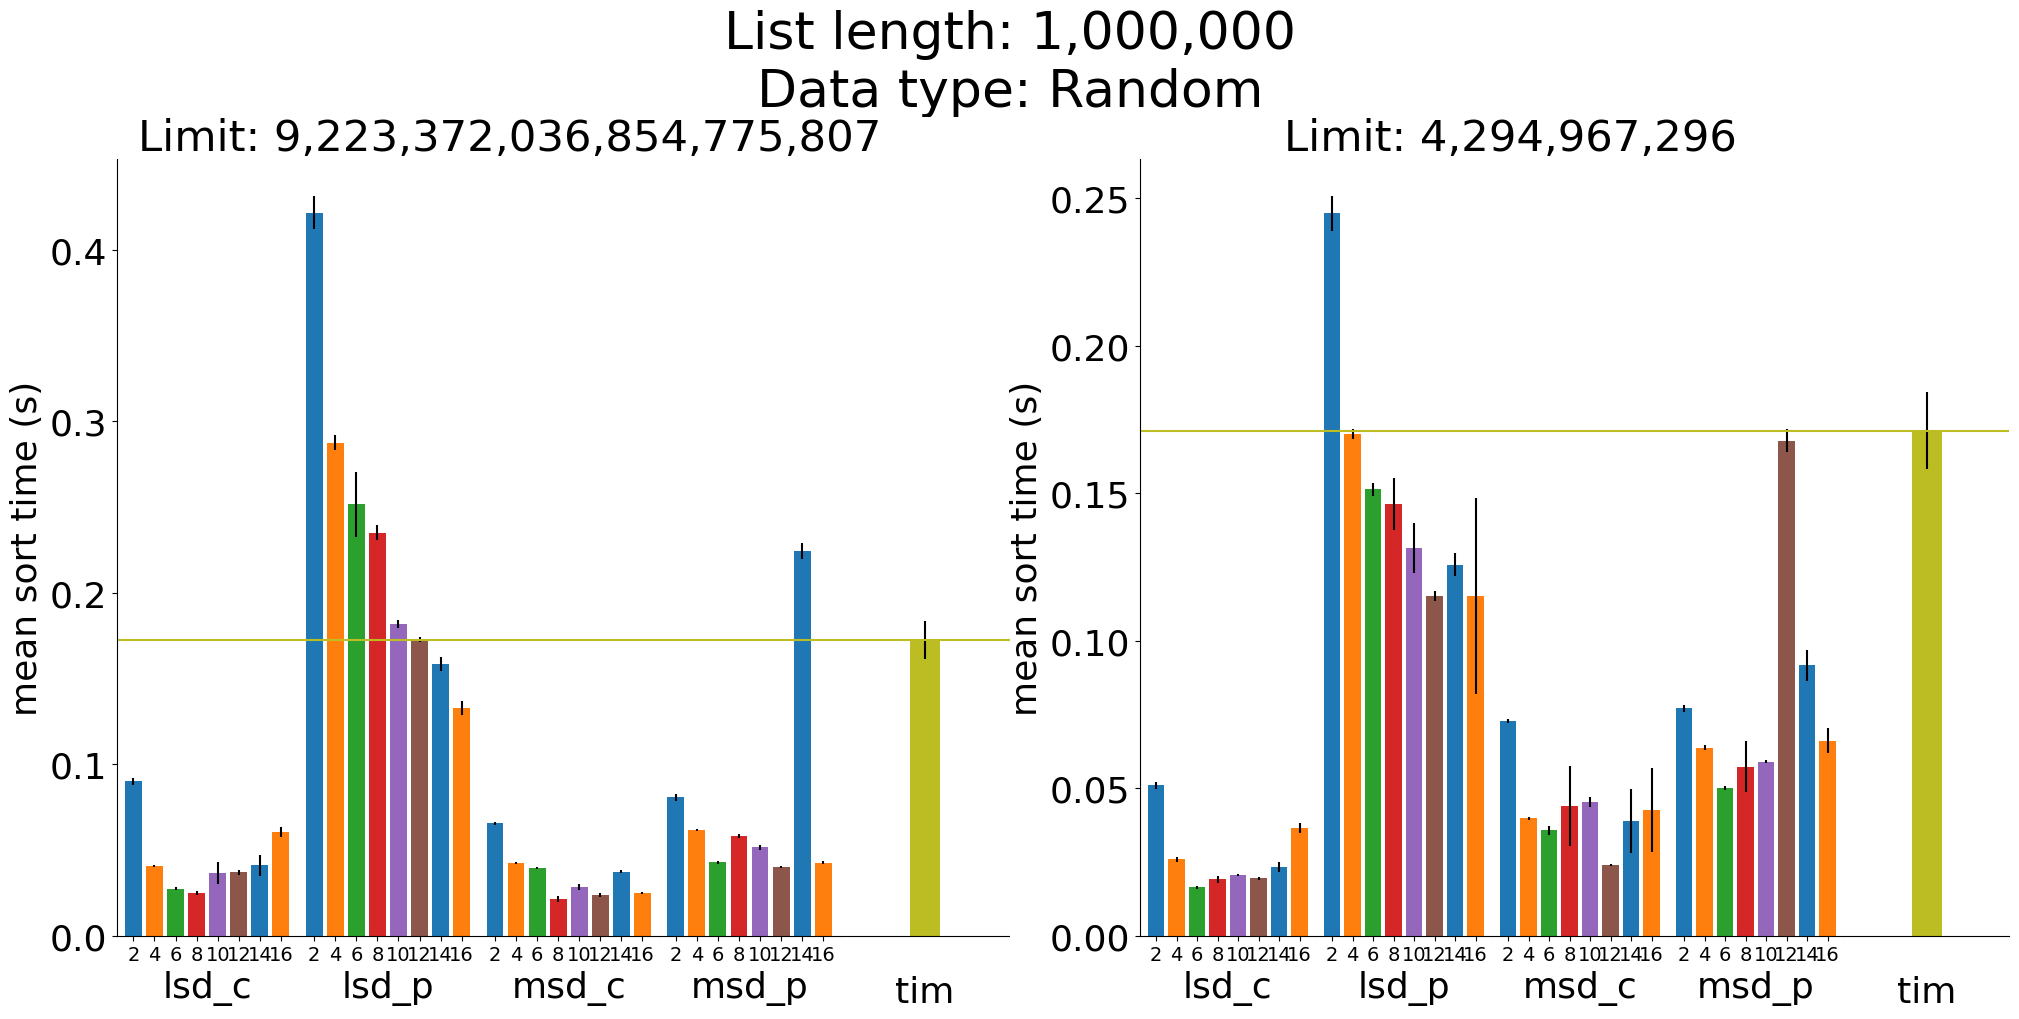
\includegraphics[ draft=false,height=6cm]{lrg_Random_0.png}
			\hspace{0.5cm}
			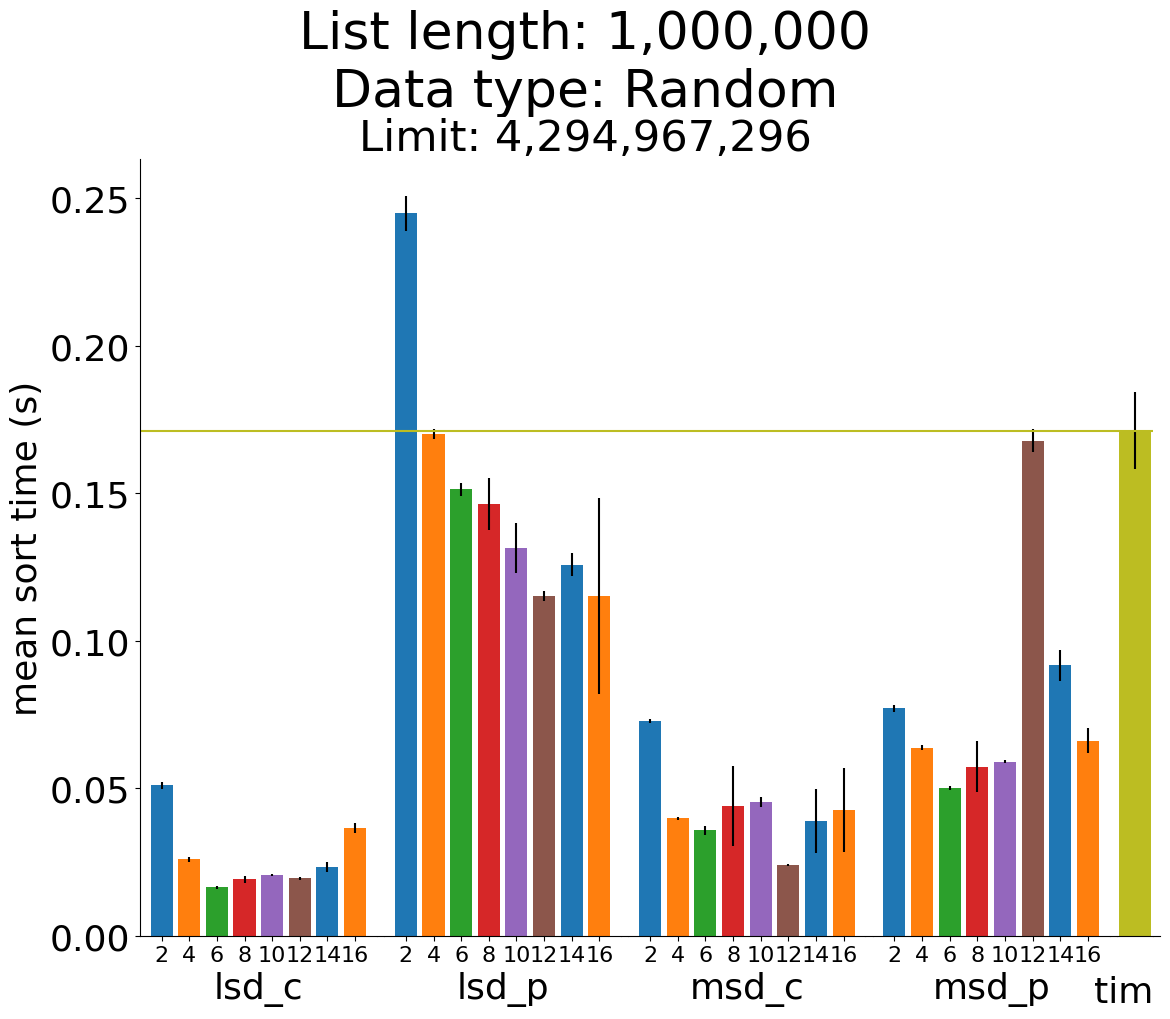
\includegraphics[ draft=false,height=6cm]{lrg_Random_1.png}
			}
			\captionof{figure}{Sort times for categorical tests, List length, data type and maximum integer identified above, Sort method and base (2-16) listed below}
			\label{fig:lrg_Random_0}

			
	\end{table}
	\myparagraph{Random}
	Random data also was used for the continuous tests and as expected, the results show similar results to the previous continuous tests for comparisons between the bases of each algorithm. 
	\par
	When comparing the algorithms against one another and timsort, the random data shows that all implementations of counting sort perform faster than timsort, as well as at least one base of each iteration of pigeonhole sort. The difference between the comparison-based nature of timsort and non-comparison-based radix sort is highlighted by observing LSD\textunderscore C for list length 1,000,000 (shown in \autoref{fig:lrg_Random_0}); Timsort completes sorting in roughly $0.17s$ regardless of integer limit whereas LSD\textunderscore C sees smaller run times for smaller integer limits, showing the benefits of the fewer digits requiring counting sort in contrast with the lack of any reduction in the number of comparisons timsort must make.
	\myparagraph{Few Unique}
	Data containing few unique values was intended to simulate sorting a series of discrete values, a potential real world usage of the algorithm. \autoref{fig:rnd-fu-diff} shows the percentage difference in sort time between sorting random and few unique data where each item is the average difference of all bases and a positive value indicates Few unique was faster. It shows there is typically a negligible difference between the two with the exception of certain higher data limits in longer lists for MSD sorts, particular counting sort. This may be due to the large number of identical items preventing insertion sort and only causes 10\% difference from random data.

	\begin{table}[h]
		\centering
		\makebox[\linewidth]{
			\centering
			\begin{minipage}[h]{.55\linewidth}
				\hspace{.05\linewidth}
				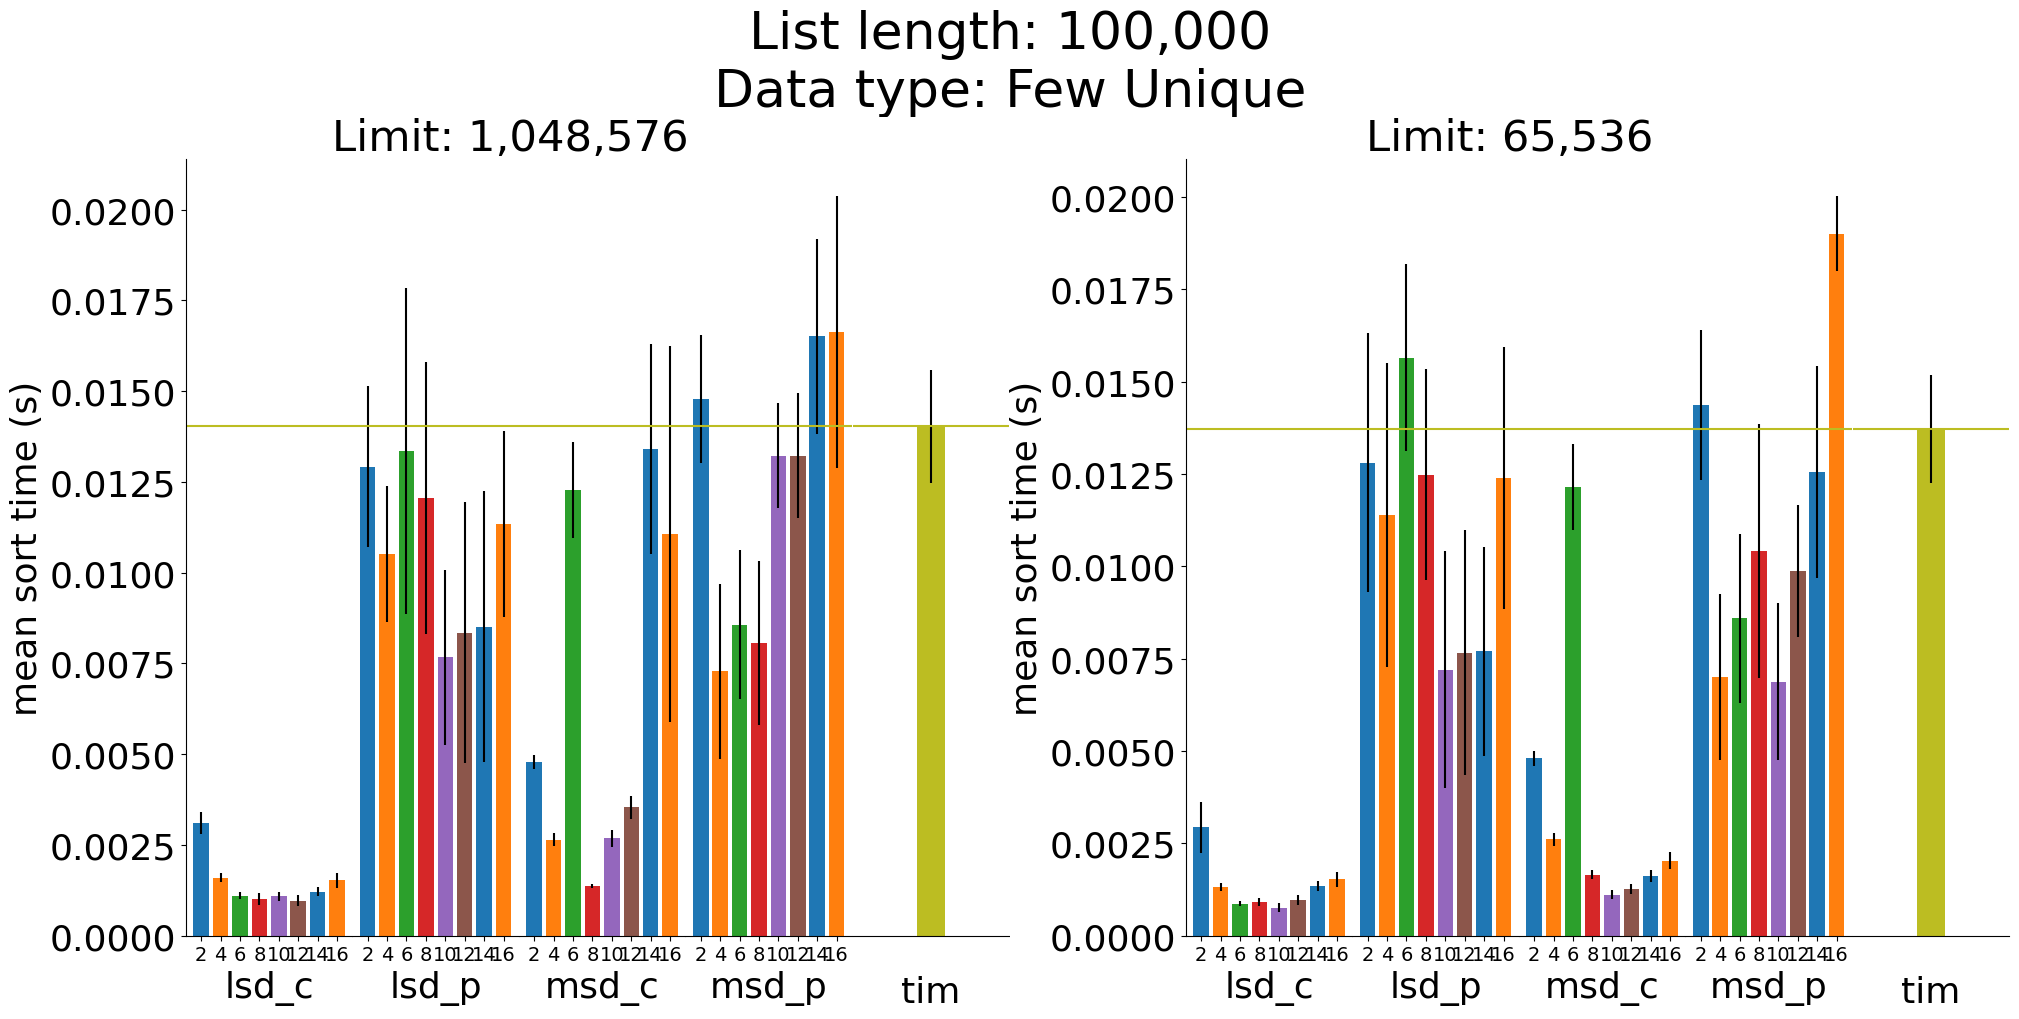
\includegraphics[ draft=false, width=.9\linewidth]{med_Few_Unique_1.png}
				\captionof{figure}{categorical tests for few unique data}
			\end{minipage}%
			\hspace{0.5cm}
			\begin{minipage}[h]{.55\linewidth}
				\resizebox{\columnwidth}{!}{%
					\begin{tabular}{llrrrrr}
						\toprule
						items & int size & lsd c & lsd p & msd c & msd p & timsort \\
						\midrule
						\multirow[t]{4}{*}{10000} & large & -9.5\% & 0.3\% & 2.3\% & 3.3\% & 6.9\% \\
						& med & -7.2\% & 6.1\% & 3.0\% & 3.6\% & 5.3\% \\
						& small & -3.4\% & 7.6\% & 6.3\% & 1.8\% & 1.1\% \\
						& tiny & -1.8\% & -0.3\% & 0.8\% & 6.5\% & 1.8\% \\
						\cline{1-7}
						\multirow[t]{4}{*}{100000} & large & 4.7\% & -23.1\% & 18.2\% & 7.1\% & 5.2\% \\
						& med & 7.2\% & -10.4\% & 10.1\% & 9.0\% & 5.1\% \\
						& small & 1.7\% & 2.1\% & 2.0\% & 16.4\% & 3.1\% \\
						& tiny & 0.9\% & -5.6\% & 11.8\% & 1.0\% & 4.8\% \\
						\cline{1-7}
						\multirow[t]{4}{*}{1000000} & large & 8.8\% & -1.0\% & -124.9\% & 10.4\% & 7.0\% \\
						& med & 8.5\% & -6.3\% & -20.1\% & -48.6\% & 3.9\% \\
						& small & 0.9\% & 7.5\% & 0.0\% & 51.2\% & 2.5\% \\
						& tiny & 2.9\% & 23.9\% & -33.7\% & 20.2\% & 4.6\% \\
						\cline{1-7}
						\multirow[t]{1}{*}{} & mean & 1.1\% & 0.1\% & -10.4\% & 6.8\% & 4.3\% \\
						\bottomrule
					\end{tabular}
				}
				\captionof{figure}{Comparison of few unique and random data, using average between equivalent bases}
				\label{fig:rnd-fu-diff}
			\end{minipage}
		}
	\end{table}
	
	\myparagraph{Nearly sorted}
	This data type was selected to make a comparison between algorithms in a situation where timsort is at an advantage. As stated in the source code for timsort \cite{listsort}, the algorithm iterates over the input, continuously identifying sorted sequences and merging them with the already sorted items and as such it is highly efficient at sorting this data which is essentially a series of sorted sequences within a larger list.
	\par
	\pagebreak
	The graphs shown in \autoref{fig:lrg_Nearly_Sorted_nolp_0} and \autoref{fig:sml_Nearly_Sorted_nolp_1} have been pruned to omit all of LSD\textunderscore P as well as bases 2, 14 and 16 as the results for these algorithms are much slower than timsort and stretch the axis, making the graph unreadable. The remaining data is representative of all tests of this data type, with timsort performing exceptionally well compared to radix sort and being faster in every situation except on lists of 10,000 items where certain bases of MSD\textunderscore P and LSD\textunderscore C are a fraction faster.  	
	\autoref{fig:rnd-ns-diff} Contains the difference in run time between Random and nearly sorted lists, it shows Whilst timsort benefits from a 94\% decrease in run time when performed on nearly sorted lists compared to random, radix sort does not see the same benefit, though there is variation base on the implementation used. MSD sorts benefit from nearly sorted lists due to their use of insertion sort which completes in $\mathcal{O}\textit{(n)}$ time on sorted lists. LSD sorts don't us this method and so don't see much benefit. The discrepancy between pigeonhole and counting sort may be due to optimizations in PyPy involving moving items from one list into another in the same order, and there is some evidence for this such as LSD\textunderscore P having larger speed gains at smaller integer limits.

	\begin{table}[h]
		\centering
		\makebox[\linewidth]{
			\begin{minipage}[h]{.5\linewidth}
				\hspace{.05\linewidth}
				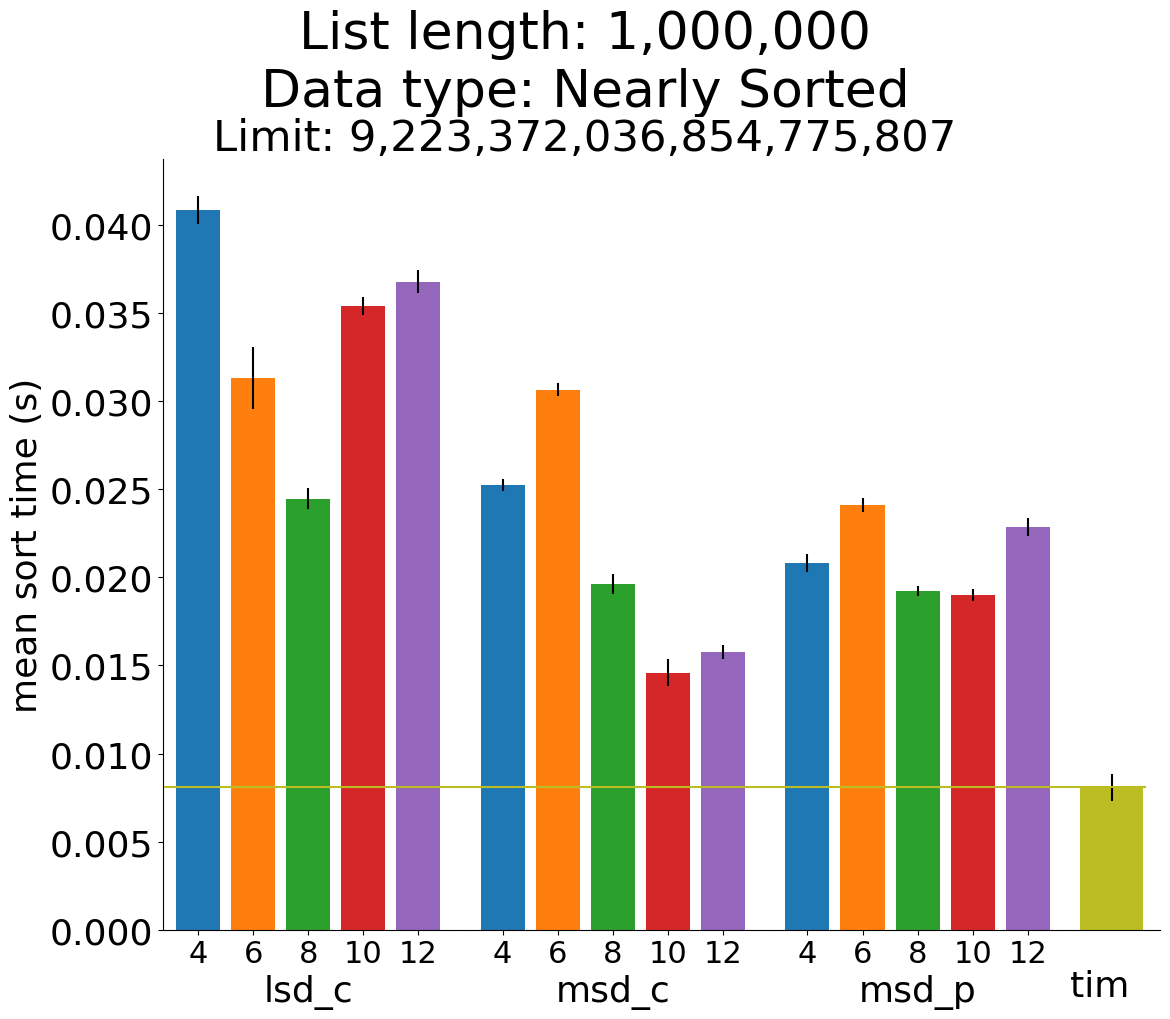
\includegraphics[draft=false, width=.9\linewidth]{lrg_Nearly_Sorted_nolp_0.png}
				\captionof{figure}{Nearly sorted data test with LSD\textunderscore P, bases 2, 14, 16 pruned}
				\label{fig:lrg_Nearly_Sorted_nolp_0}				

				
			\end{minipage}
			\hspace{0.25cm}
			\begin{minipage}[h]{.6\linewidth}
				\resizebox{\columnwidth}{!}{%
					\begin{tabular}{llrrrrr}
						\toprule
						items & int size & lsd c & lsd p & msd c & msd p & timsort \\
						\midrule
						\multirow[t]{4}{*}{10000} & large & -3.1\% & -8.4\% & -1.3\% & 32.3\% & 91.9\% \\
						& med & -3.6\% & -9.7\% & 17.5\% & 52.0\% & 92.0\% \\
						& small & -4.5\% & -5.1\% & 0.9\% & 43.5\% & 92.2\% \\
						& tiny & -1.8\% & -3.9\% & 15.1\% & 39.6\% & 92.0\% \\
					   \cline{1-7}
					   \multirow[t]{4}{*}{100000} & large & -0.2\% & 6.7\% & 8.6\% & 27.5\% & 94.4\% \\
						& med & -1.6\% & 10.8\% & 19.6\% & 43.1\% & 94.3\% \\
						& small & -3.7\% & 20.0\% & 16.4\% & 39.0\% & 94.3\% \\
						& tiny & -7.2\% & 32.4\% & 14.0\% & 31.1\% & 95.0\% \\
					   \cline{1-7}
					   \multirow[t]{4}{*}{1000000} & large & 0.3\% & 6.1\% & 35.4\% & 54.7\% & 95.3\% \\
						& med & 1.4\% & 0.4\% & 23.0\% & 47.0\% & 95.1\% \\
						& small & -1.4\% & 22.6\% & 14.7\% & 40.5\% & 95.2\% \\
						& tiny & 11.9\% & 32.9\% & 28.7\% & 41.8\% & 98.6\% \\
						\cline{1-7}
						\multirow[t]{1}{*}{} & mean & -1.1\% & 8.7\% & 16.0\% & 41.0\% & 94.3\% \\
						\bottomrule
					\end{tabular}
				}
				\captionof{figure}{Comparison of Nearly sorted and random data, using average between equivalent bases. Positives indicate nearly sorted is faster}
				\label{fig:rnd-ns-diff}

			\end{minipage}

		}
		\\	
		\vspace{1cm}

		\makebox[\linewidth]{
		\begin{minipage}[h]{.5\linewidth}				
			\hspace{.05\linewidth}
			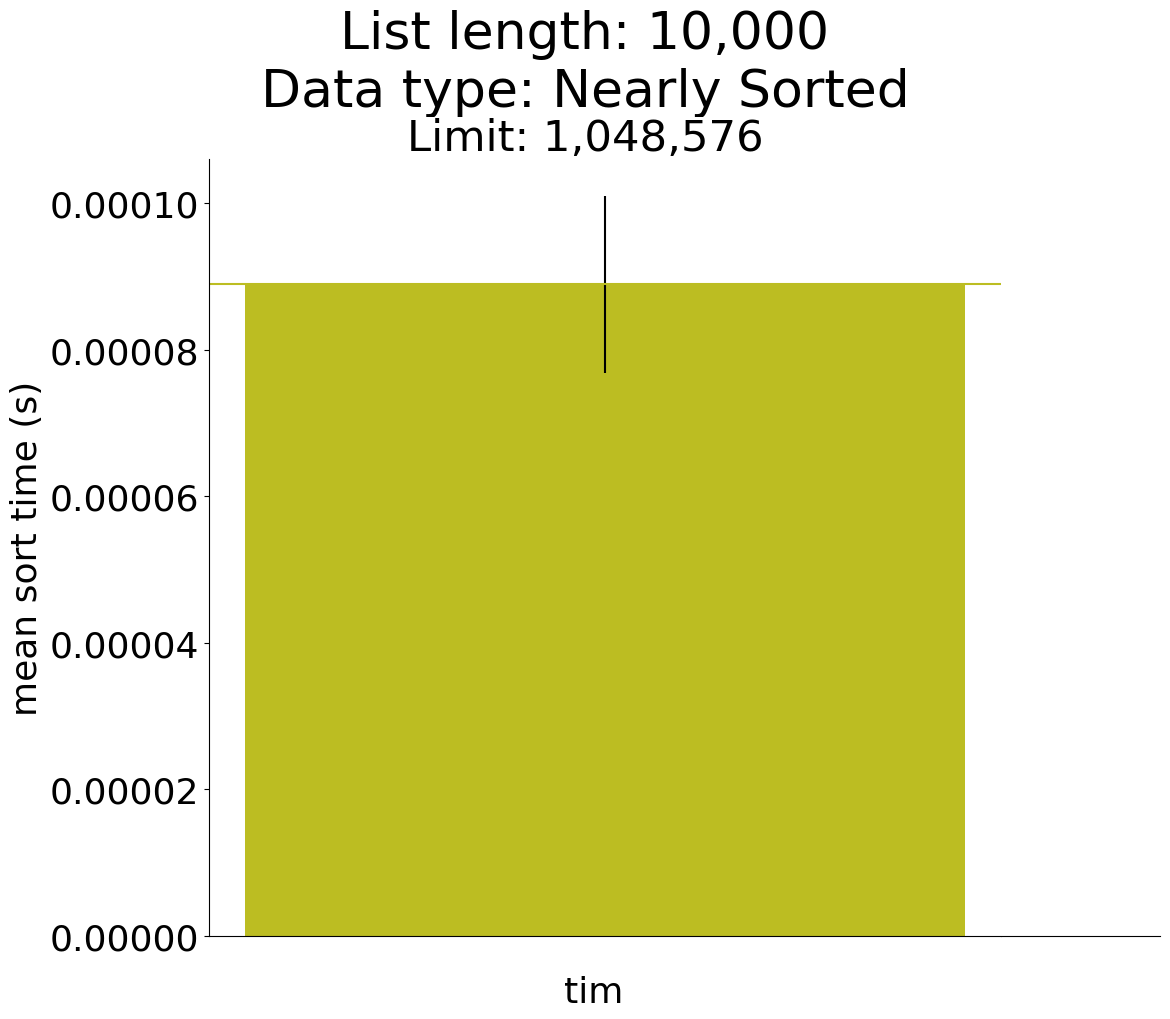
\includegraphics[draft=false, width=.9\linewidth]{sml_Nearly_Sorted_nolp_2.png}
		\end{minipage}
		\hspace{0.25cm}
		\begin{minipage}[h]{.6\linewidth}	
			\centering			
			\resizebox{.8\columnwidth}{!}{%
			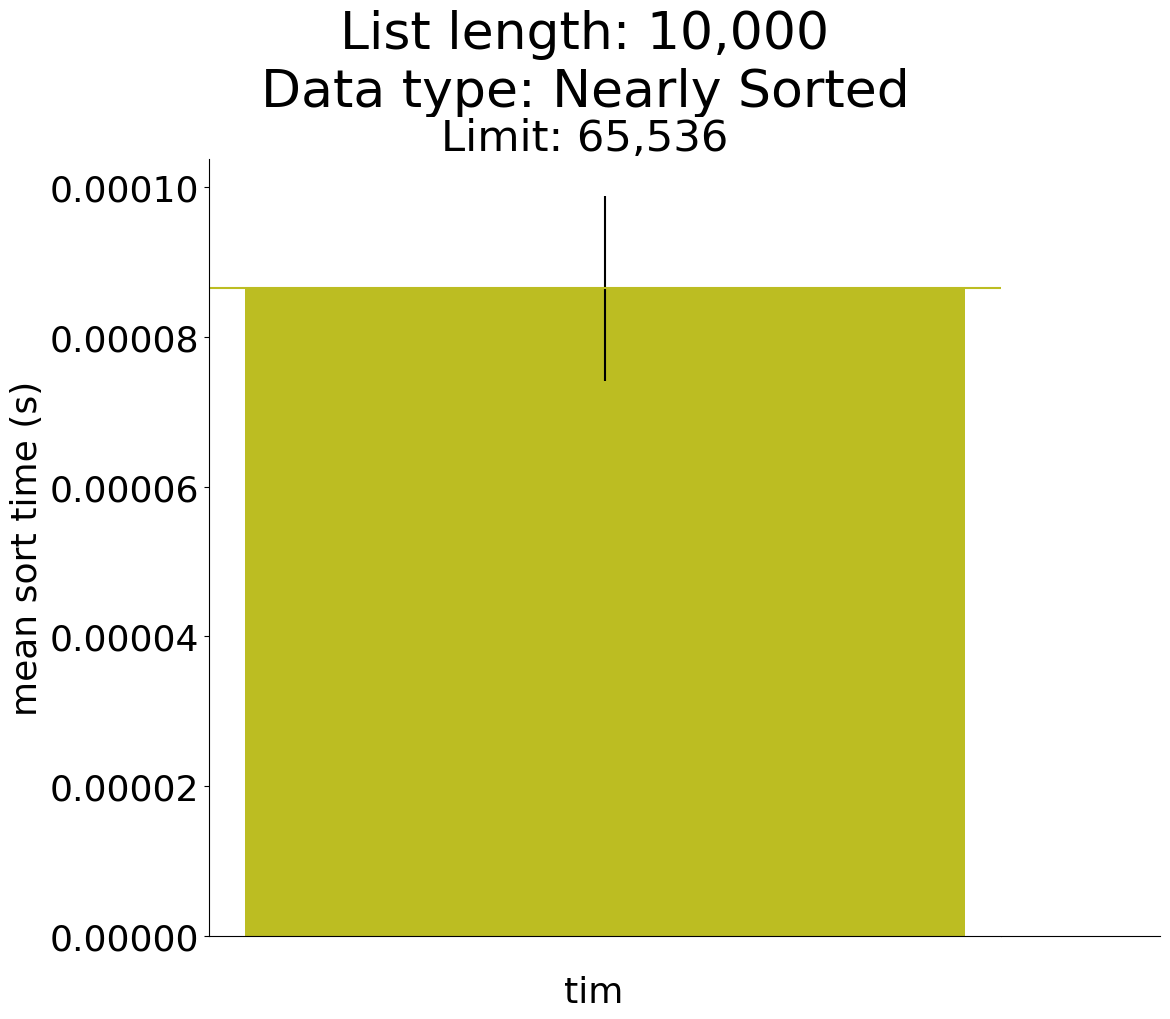
\includegraphics[draft=false, width=.9\linewidth]{sml_Nearly_Sorted_nolp_3.png}
			}
		\end{minipage}
		}
		\captionof{figure}{Nearly sorted data test showing list length 10,000}
		\label{fig:sml_Nearly_Sorted_nolp_1}

	\end{table}
	% \begin{table}[h]
	% 	\centering

	% \end{table}


	\subsubsection{Testing evaluation}
	The goal of testing was to produce data suitable for analysis to decide which base is the best for each implementation and then to decide which of the implementations,if any, is best for replacing timsort. The main limitations of the tests are that it is not possible to test every permutation of all the factors affecting performance of the algorithms, such as integer digits and list length, and that the testing was all completed on one machine and therefore may not necessarily be applicable to other machines. 
	\par For these reasons, and to attempt to fairly evaluate the lists in the widest range of circumstances, the analysis to identify the best base relies upon data that has been normalized within each group containing a list length, maximum integer size, data type, and radix sort implementation. This normalized data allows the comparison of input types that vary wildly in terms of sorting time such as lists containing 10,000 and 1,000,000 items.
	\par
	\autoref{fig:averageresults} contains the normalized data, representative of each base's performance compared to peers of the same radix sort implementation and ranked from fastest to slowest with a negative result for time indicating the base was faster than average.

	\begin{table}[h]
		\centering
		\begin{tabular}{c|cl|cl|cl|cl}
			\toprule
			\multicolumn{1}{c}{}& \multicolumn{2}{c}{lsd c} & \multicolumn{2}{c}{lsd p} & \multicolumn{2}{c}{msd c} & \multicolumn{2}{c}{msd p} \\
			 \midrule
			 \multicolumn{1}{c}{rank} & base & \multicolumn{1}{c}{time} & base & \multicolumn{1}{c}{time} & base & \multicolumn{1}{c}{time} & base & \multicolumn{1}{c}{time} \\
			\midrule
			1 & 8 & -0.721 & 12 & -0.728 & 8 & -0.611 & 6 & -0.637 \\
			2 & 6 & -0.689 & 10 & -0.678 & 10 & -0.554 & 8 & -0.372 \\
			3 & 12 & -0.653 & 14 & -0.523 & 12 & -0.325 & 4 & -0.327 \\
			4 & 10 & -0.623 & 8 & -0.319 & 4 & -0.312 & 10 & -0.319 \\
			5 & 14 & -0.139 & 6 & -0.048 & 6 & -0.022 & 12 & -0.232 \\
			6 & 4 & \,\,0.008 & 4 & \,\,0.116 & 16 & \,\,0.332 & 2 & \,\,0.171 \\
			7 & 16 & \,\,0.998 & 16 & \,\,0.843 & 14 & \,\,0.409 & 14 & \,\,0.327 \\
			8 & 2 & \,\,1.819 & 2 & \,\,1.338 & 2 & \,\,1.082 & 16 & \,\,1.389 \\
			\bottomrule
			\end{tabular}
			\captionof{table}{Comparison of the performance of the numerical bases for each sort method\newline Shows average normalized sort times in each list length, maximum integer and data type}
			\label{fig:averageresults}
		\end{table}

	Selection of the most suitable base for each method was made by combining the information in \autoref{fig:averageresults} and the results of the continuous tests, the choices and the justification for each are detailed below. 
		
	\begin{description}
		\item[LSD Counting - 10] Whilst \autoref{fig:averageresults} shows bases 8 and 6 perform better on average than 10 and 12, the results from the continous tests show that as the input list length increases the lower 2 bases decrease in performance and as the input limit increases base 6 slows relative to 8, 10 and 12. Base 10 was selected over 12 based on the continous test results for input list length which shows 10 as being marginally faster. This test was used because the categorial results are so similar, with a difference of only $0.03$ in 12's favour not providing enough justification for it's selection.
		\item[LSD Pigeonhole - 12] Base 12 has the lowest average sort time in \autoref{fig:averageresults} and performs at least as well as or better than 10 in the continuous tests.
		\item[MSD Counting - 10] Base 8 performs the best based on the results in \autoref{fig:averageresults}, but performs poorly in the continous test for list length.
		\item[MSD Pigeonhole - 6] No other base seems viable based on \autoref{fig:averageresults}, and base 6 is among the best performers in the continous test for list length.
	\end{description}
	\par
	Using the data produced during the categorical testing process, the 4 selected bases can be isolated and compared with timsort, the tables below show the average normalized time for each alongside the average rank 1-5.
	\par
	\autoref{fig:datatype} compares the algorithms with a separation between data type (Few Unique data was omitted as it shows similar results to Random), it highlights that for nearly sorted data timsort significantly out-performs radix sort, however it is actually the worst performer when sorting random data. The table also shows an order amongst the radix sort implementations, from best to worst this is: LSD Counting, MSD counting, MSD Pigeonhole, LSD Pigeonhole. In general, the data for the performance across all categories follows this trend, though it is not universally true.
	\begin{table}[h]
		\centering
		\begin{tabular}{c|cl|cl|cl}
			\toprule
			\multicolumn{1}{c}{data type} & \multicolumn{2}{c}{Few Unique} & \multicolumn{2}{c}{Nearly Sorted} & \multicolumn{2}{c}{Random} \\
			\midrule
			\multicolumn{1}{c}{} & rank & times & rank & times & rank & times \\
			\midrule
			lsd c  & \,\,1.25  & -1.02  & \,\,2.42  & -0.61  & \,\,1.25  & -0.99 \\
			lsd p  & \,\,3.5  & \,\,0.17  & \,\,4.83  & \,\,1.68  & \,\,3.75  & \,\,0.35 \\
			msd c  & \,\,2.08  & -0.7  & \,\,3.08  & -0.22  & \,\,1.75  & -0.81 \\
			msd p  & \,\,3.25  & -0.03  & \,\,3.58  & \,\,0.12  & \,\,3.33  & -0.18 \\
			timsort  & \,\,4.92  & \,\,1.58  & \,\,1.08  & -0.97  & \,\,4.92  & \,\,1.62 \\
			\bottomrule
			\end{tabular}
		
			\captionof{table}{Average rank 1-5 and normalized time with separation between data type}
			\label{fig:datatype}
	\end{table}

	
	
	
\pagebreak
\printbibliography
\end{document}